%
% Einfache LaTeX-Vorlage f�r Arbeiten am Lehrstuhl Kranzlm�ller / MNM-Team
% - optimiert f�r die Arbeit mit g�ngigen LaTeX-Editoren
% - funktioniert ohne Makefile und Anpassungen der LaTeX-Verzeichnisstruktur
% - verwendet Komaskript f�r ein (nach europ�ischen Gepflogenheiten) sch�neres Layout
% 
% v1, 2007 (Michael Brenner)
% Diese Version: v1.1, 2012 (Michael Brenner)
% Diese Version: v1.2, 2017 (Michael Brenner)
% 


\documentclass[bibliography=totoc,listof=totoc,BCOR=5mm,DIV=12]{scrbook} % Rand f�r Bindung: 5mm / falls Index verwendet, erg�nze "index=totoc" zu den Optionen 
\usepackage[latin1]{inputenc} % Umlaute im Text
\usepackage{graphicx} % Einf�gen von Grafiken  - f�r PDF-Latex: .pdf und .png (.jpg m�glich, sollte aber vermieden werden)
\usepackage{url}           % URL's (z.B. in Literatur) sch�ner formatieren
\usepackage{hyperref} % sorgt f�r f�r Hyperlinks in PDF-Dokumenten
\usepackage{color}
\usepackage{listings}
\usepackage{color}
\usepackage{tabularx}
\usepackage{booktabs}
\usepackage{ltablex}
\usepackage[toc,page]{appendix}
\usepackage[]{algorithm2e}
\newcommand*{\Appendixautorefname}{appendix}

\definecolor{lightgray}{rgb}{0.5,0.5,0.5}
\definecolor{gray}{rgb}{0.5,0.5,0.5}
\definecolor{mauve}{rgb}{0.58,0,0.82}

\SetAlCapSkip{1em}

\lstset{frame=tb,
  language=C++,
  aboveskip=6mm,
  belowskip=6mm,
  showstringspaces=false,
  columns=flexible,
  basicstyle={\small\ttfamily},
  numbers=left,
  numbersep=5pt,
  numberstyle=\tiny\color{gray},
  keywordstyle=\color{blue},
  commentstyle=\color{lightgray},
  stringstyle=\color{mauve},
  breaklines=true,
  breakatwhitespace=true,
  tabsize=3
}

\newtheorem{defi}{Definition}[chapter]
\newtheorem{lemma}{Observation}[chapter]

\usepackage{array}
\setlength\extrarowheight{2pt}

\graphicspath{{./Bilder/}}

%
% der Befehl \hypenation versteht keine Sonderzeichen, also weder �
% noch "a noch \"a. W�rter die derartige Zeichen enthalten m�ssen
% direkt im Text getrennt werden, z.B. W�r\-ter
%
\hyphenation{Ma-nage-ment}
\hyphenation{Ma-nage-ment-agent}
\hyphenation{Ma-nage-ment-agent-en}
\hyphenation{Ma-nage-ment-ar-chi-tek-tur}
\hyphenation{Ma-nage-ment-ar-chi-tek-tu-ren}
\hyphenation{Ma-nage-ment-an-wen-dung}
\hyphenation{Ma-nage-ment-an-wen-dung-en}
\hyphenation{Ma-nage-ment-an-for-der-ung}
\hyphenation{Ma-nage-ment-funk-ti-on}
\hyphenation{Ma-nage-ment-funk-ti-onen}
\hyphenation{Ma-nage-ment-kon-zep-te}
\hyphenation{Ma-nage-ment-res-source}
\hyphenation{Ma-nage-ment-in-for-ma-ti-on}
\hyphenation{Ma-nage-ment-res-sour-cen}
\hyphenation{ma-nage-ment-re-le-vante}
\hyphenation{ma-nage-ment-sy-stem}
\hyphenation{ma-nage-ment-sy-steme}
\hyphenation{Ma-nage-ment-in-stru-men-tie-rung}
\hyphenation{Ma-nage-ment-platt-form}
\hyphenation{Sys-te-men}
\hyphenation{Sys-tem-um-ge-bun-gen}
\hyphenation{Sys-tem-ma-nage-ment}
\hyphenation{DHCP}
\hyphenation{Ma-nage-ment-diszi-plinen}
\hyphenation{System-management-architekturen}
\hyphenation{Verwendungs-nachweise}
\hyphenation{Video-einricht-ungen}
\hyphenation{Res-source}
\hyphenation{Res-sourcen}
\hyphenation{Grund-anwendung}
\hyphenation{Grund-anwendungen}
\hyphenation{Basis-anwendung}
\hyphenation{Core}
\hyphenation{Kom-mu-ni-ka-ti-on}
\hyphenation{De-sign-ent-schei-dung}
\hyphenation{Sprung-ad-res-sen}
\hyphenation{Klas-si-fi-ka-ti-on}
\hyphenation{Schreib-recht}
\hyphenation{Be-nut-zer-zer-ti-fi-kat}
\hyphenation{Bau-stein-ent-wi-ckler}
\hyphenation{ad-mi-ni-stra-ti-ve}

 % in dieses File kommen W�rter die Latex nicht richtig trennt

\begin{document}

% ---------------------------------------------------------------
\frontmatter % Titelbl�tter und Erkl�rung jeweils spezifisch f�r die jeweilige Uni einbinden
    %%%%%%%%%%%%%%%%%%%%%%%%%%%%%%%
% erste Seite

\thispagestyle{empty}

\begin{center}

\vspace*{-2cm}

{\Huge INSTITUT F�R INFORMATIK\\[1mm]}
DER LUDWIG--MAXIMILIANS--UNIVERSIT�T M�NCHEN\\

\vspace*{1cm}


\includegraphics[width=0.3\textwidth]{lmu_siegel}

\vspace*{2cm}

{\Large \textbf{Master's Thesis}}\\ % oder Fortgeschrittenenpraktikum, Master's Thesis, Bachelorarbeit etc.

\vspace{2.0cm}
{\Huge \textbf{C++ Graph Concepts for}}\\
\vspace*{3mm}
{\Huge \textbf{Partitioned Global Address Space}}\\
\vspace*{20mm}

{\LARGE Stefan Effenberger} % Name des Autors

\vspace{3cm}
\end{center}

\newpage

%%%%%%%%%%%%%%%%%%%%%%%%%%%%%%%
% zweite Seite

\thispagestyle{empty}
\cleardoublepage

%%%%%%%%%%%%%%%%%%%%%%%%%%%%%%%
% dritte Seite (Kopie der ersten)

\thispagestyle{empty}

\begin{center}

\vspace*{-2cm}

{\Huge INSTITUT F�R INFORMATIK\\[1mm]}
DER LUDWIG--MAXIMILIANS--UNIVERSIT�T M�NCHEN\\

\vspace*{1cm}


\includegraphics[width=0.3\textwidth]{lmu_siegel}

\vspace*{2cm}

{\Large \textbf{Master's Thesis}}\\ % oder Fortgeschrittenenpraktikum, SEP etc.

\vspace{2.0cm}
{\Huge \textbf{C++ Graph Concepts for}}\\
\vspace*{3mm}
{\Huge \textbf{Partitioned Global Address Space}}\\
\vspace*{20mm}

{\LARGE Stefan Effenberger} % Name des Autors
\vspace{2cm}

\parbox{1cm}{
\begin{large}
\begin{tabbing}
Aufgabensteller: \hspace{.5cm} \=Prof. Dr. Dieter Kranzlm�ller\\[2mm]
Betreuer:
\>Tobias Fuchs\\[5mm]
Abgabetermin: \> \textcolor{red}{ADD DATE}\\
\end{tabbing}
\end{large}}\\
\vspace{5mm}

\end{center}
 % Titelbl�tter LMU - auskommentieren falls TUM-Arbeit
%    % Richtlinien, siehe http://wwwpa.in.tum.de/generell/Abschlussarbeitsform.html
%
%%%%%%%%%%%%%%%%%%%%%%%%%%%%%%%


% Deckblatt

\thispagestyle{empty}

\begin{center}
    
\includegraphics[width=3cm]{tum-logo}\\
    \vspace{.5cm}
% "Technische Universit�t M�nchen" oder alternativ das Logo der TUM
    {\Large \sc Technische Universit�t M�nchen}\\

    \vspace{1cm}
% "Fakult�t f�r Informatik"
    {\Huge \sc Fakult�t f�r Informatik\\[1mm]}


    \vspace{2cm}
% Diplomarbeit | Master's Thesis | Bachelorarbeit in Informatik | Wirtschaftsinformatik |
    {\Large \textbf{Masterarbeit in Informatik}}\\
% Thema bzw. Titel der Arbeit  (In der Sprache, in der die Arbeit verfasst wurde)
    \vspace{2.0cm}
    {\Huge \textbf{Ein Lorem-Rahmenwerk}}\\ % bei langen Titeln ggf. Schriftgr��e auf \huge herunter setzen
    \vspace*{3mm}
    {\Huge \textbf{f�r Ipsum-Systeme}}\\
    \vspace*{3mm}
    {\Huge \textbf{-- ein Dolor-Ansatz}}\\
    \vspace{1.5cm}
% Vorname und Nachname des Bearbeiters/ der Bearbeiterin
    Vorname Nachname

    \vspace{5cm} % ggf. je nach Zeilenzahl und Schriftgr��e des Titels anpassen
    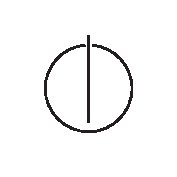
\includegraphics[width=2.4cm]{tum-info-logo}
\end{center}

\newpage

%%%%%%%%%%%%%%%%%%%%%%%%%%%%%%%
% R�ckseite Deckblatt

\thispagestyle{empty}
\cleardoublepage

%%%%%%%%%%%%%%%%%%%%%%%%%%%%%%%
% Erste Seite (Titelblatt)

\thispagestyle{empty}

\begin{center}

    
\includegraphics[width=3cm]{tum-logo}\\
    \vspace{.5cm}
    {\Large \sc Technische Universit�t M�nchen}\\


    \vspace{.5cm}

    {\huge \sc Fakult�t f�r Informatik\\[1mm]}


    \vspace{1cm}

    {\Large \textbf{Diplomarbeit in Informatik}}\\ % oder SEP etc.

% Thema bzw. Titel der Arbeit  (In der Sprache, in der die Arbeit verfasst wurde)
    \vspace{1.5cm}
    {\huge \textbf{Ein Lorem-Rahmenwerk}}\\ % bei langen Titeln ggf. Schriftgr��e herunter setzen
    \vspace*{3mm}
    {\huge \textbf{f�r Ipsum-Systeme}}\\
    \vspace*{3mm}
    {\huge \textbf{-- ein Dolor-Ansatz}}\\

% die englische bzw. deutsche Entsprechung des Titels
    \vspace{1cm}
    {\huge \textbf{A Lorem Framework}}\\ % bei langen Titeln ggf. Schriftgr��e herunter setzen
    \vspace*{3mm}
    {\huge \textbf{for Ipsum Systems}}\\
    \vspace*{3mm}
    {\huge \textbf{-- a Dolor Approach}}\\
    \vspace{1cm}

    \parbox{1cm}{
      \begin{large}
        \begin{tabbing}
          Bearbeiter: \hspace{1.5cm}
            \=Vorname Nachname\\[2mm]
    Aufgabensteller: \>Prof. Dr. Dieter Kranzlm�ller\\[2mm]
    Betreuer: \>MNM-Team-Betreuer 1\\ % alphabetische Reihenfolge (Nachname)
    \>MNM-Team-Betreuer 2\\
    \>Externer Betreuer 1 (Firma)\\[5mm]
    Abgabedatum: \> 7. Juli 2077\\
        \end{tabbing}
      \end{large}
    }\\

    \vspace{.3cm}

    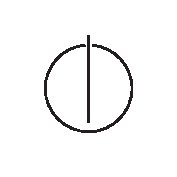
\includegraphics[width=2.4cm]{tum-info-logo}

\end{center}
 % Titelbl�tter TUM - auskommentiert lassen falls LMU-Arbeit
    \thispagestyle{empty}
    \cleardoublepage
    %
% LaTeX-Rahmen f�r Arbeiten am Lehrstuhl Hegering
%
% Harald Roelle, 2001, 2002
%
% basierend auf Arbeiten von Helmut Reiser, Boris Gruschke und Stephen Heilbronner
%

\newpage

\thispagestyle{empty}

\begin{large}

\vspace*{2cm}

\noindent
Hiermit versichere ich, dass ich die vorliegende Masterarbeit
selbst�ndig verfasst und keine anderen als die angegebenen Quellen
und Hilfsmittel verwendet habe.

\vspace{2cm}

\noindent
M�nchen, den \textcolor{red}{ADD DATE}

\vspace{3cm}

\hspace*{7cm}%
\dotfill\\
\hspace*{8.5cm}%
\textit{(Unterschrift des Kandidaten)}

\end{large}
 % Erkl�rung (Arbeit selbstst�ndig verfasst) - auskommentieren falls TUM-Arbeit
%    \begin{large}

\vspace*{2cm}
\noindent
Ich versichere, dass ich diese Masterarbeit % (bzw. Master's Thesis)
selbst�ndig verfasst und nur die angegebenen Quellen und Hilfsmittel verwendet habe.

\vspace{2cm}

\noindent
M�nchen, den 7. Juli 2077

\vspace{3cm}

\hspace*{7cm}%
\dotfill\\
\hspace*{8.5cm}%
\textit{(Unterschrift des Kandidaten)}

\end{large}
 % Erkl�rung (Arbeit selbstst�ndig verfasst) - auskommentiert lassen falls LMU-Arbeit
    \thispagestyle{empty}
    \cleardoublepage
    \vspace*{2cm}

\begin{center}
    \textbf{Abstract}
\end{center}

\vspace*{1cm}

\noindent Hier steht eine kurze Zusammenfassung der Arbeit. Sie darf auf gar keinen Fall
l�nger als eine Seite sein, ca. eine drittel bis eine halbe Seite ist optimal.

 % Abstract
    \thispagestyle{empty}
    \tableofcontents % Inhaltsverzeichnis

% ---------------------------------------------------------------
\mainmatter % die eigentliche Arbeit

\chapter{Introduction}
Many scientific projects are largely enabled by simulation. Because such simulations often require huge computational capabilities, single compute nodes with a shared-memory architecture cannot provide enough computation power and storage for numerous cases. For this reason, in High Performance Computing (HPC), work is distributed among multiple interconnected nodes to facilitate the solving of large problems in a timely manner. Since processors cannot directly access the memory of other nodes, the traditional programming model for such systems requires programmers to explicitly distribute data between nodes via message passing. This imposes high demands on the programming skills of scientists who might not have a background in computer science.

Therefore, with the Partitioned Global Address Space (PGAS) model, a new approach is proposed: The memory space of individual nodes in a system is unified within a global address space so that each node can directly access the memory of all other nodes. Programmers are still required to keep data access between nodes to a minimum because data transfer over an interconnect is costly. To further reduce the demands on the programmer, distributed data structures that handle data distribution and load balancing are needed.

Furthermore, data-intensive tasks have been gaining a continually growing interest in the scientific community. Traditionally, applications in HPC follow a computation-centric approach by solving numerical algorithms in the fastest possible way. As ``Big Data'' is becoming increasingly important in scientific projects, a shift towards more data-oriented applications can be observed in recent HPC projects \cite{fusionfs}. This trend requires distributed data structures that allow for the storage of large amounts of irregular data and cater to the needs of ever-changing dynamic data.

\section{Problem statement}
Data can be represented in numerous ways. The most generic form of data representation is enabled by \textit{graphs}. A graph $G(V, E)$ is a pair with a set of vertices V and a set of edges E that connect the vertices. This allows for the representation of data and its relationships in regular as well as irregular patterns.

On distributed machines, graph data structures can be implemented using a variety of different characteristics. This has led to many different implementations - usually a new implementation for each algorithm - which are hardly compatible with each other. To overcome this situation, generic programming abstractions to facilitate reuse of existing code and to lower the demands on programmers are needed.

As of today, no generic graph abstractions implementing the PGAS model exist. This work therefore aims to provide a graph abstraction for C++ containers that allows for the implementation of arbitrary graph algorithms following the PGAS model on distributed memory machines.

\section{Scope and objectives}
In this work, C++ concepts for graph containers following the PGAS model is presented. The graph concepts are meant to provide a generic framework for the programming of arbitrary graph algorithms in the context of distributed machines and especially the Partitioned Global Address Space model. This means that it meets the following requirements:

\begin{itemize}  
\item Native support for one-sided communication
\item Support for the programming of synchronous graph algorithms
\item Support for the programming of asynchronous graph algorithms
\item Portability across platforms and portable efficiency
\end{itemize}

Furthermore, this work provides concepts for the dynamic allocation of graph data across multiple machines with a focus on optimized data locality.

A reference implementation is then used to verify the usability, correctness and universality of the given concepts.

\chapter{Background}
This chapter covers some fundamental background knowledge needed for a better understanding of the following chapters of this thesis. Only explanations directly relevant to the topics of this thesis are provided.

Since the result of this work are C++ concepts, some important language expressions and concepts are firstly discussed, along with a description of the Standard Template Library \cite{stl} on which concepts this work is built upon. The reader is then introduced to the domain of High Performance Computing which is the main application area of this work. A brief overview of the Partitioned Global Address Space programming model is then followed by a description of the DASH Library \cite{dash} that serves as a framework for the reference implementation of this work.

\section{Graph representations}
This section provides a brief overview of different graph representations used in computer sciences \cite{ita}. Basically, there are two different representations with different but overlapping application areas. 

\begin{figure}[ht]
	\centering
  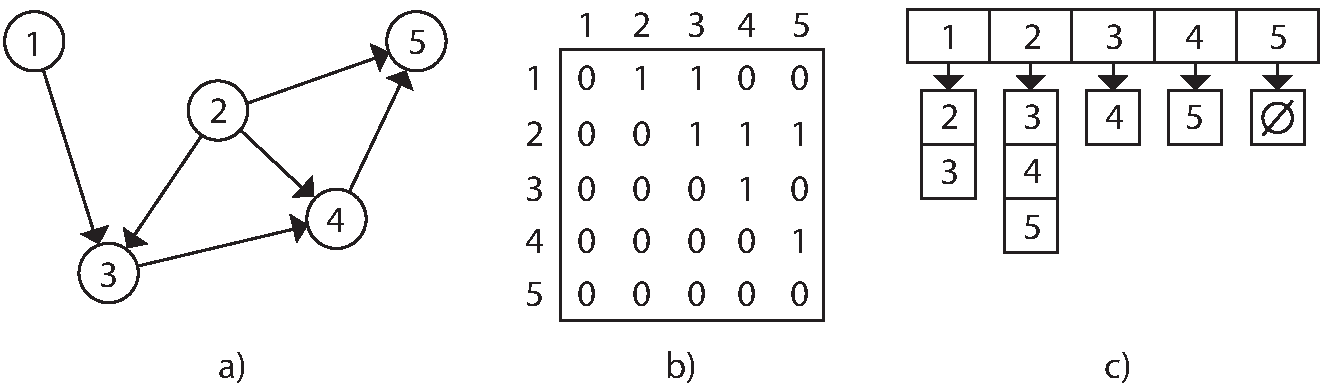
\includegraphics[width=1\textwidth]{Bilder/graph_rep.pdf}
	\caption{A directed graph (a) that is represented as an adjacency matrix (b) and as an adjacency list (c)}
	\label{graph_rep_figure}
\end{figure}

\autoref{graph_rep_figure} shows a directed graph that is represented in two ways: \textit{adjacency matrix} and \textit{adjacency list}. Both representations are also suitable for \textit{undirected} and \textit{bidirectional} graphs, but not for \textit{hypergraphs}.

\subsection{Adjacency matrix}
A graph \(G(V, E)\) with a set of vertices \(V\) and a set of edges \(E\) can be represented by a \(|V| \times |V|\) matrix \(A = a_{ij}\) using a binary edge coding: If an edge \((i, j)\) exists in the set of edges \(E\),  \(a_{ij}\) is set to 1. In all other cases, \(a_{ij}\) is set to 0.

A matrix data structure occupies a memory region for \(|V|^2\) elements regardless of the amount of edges in the graph. For large, \textit{sparse graphs}, this results in an unnecessarily high amount of required memory. A normal matrix therefore is only suitable for \textit{dense graphs}. However, matrices containing a huge amount of elements with the same content (zeros in this case) can be compressed. For example, the \textit{Compressed Sparse Row (CSR)} format \cite{sparse_linear} allows to reduce the memory consumption of sparse matrices significantly. As can be seen in \autoref{graph_rep_figure} b), directed graphs only occupy the fields at the right side of the matrix' main diagonal. For undirected graphs, fields are symmetric along the diagonal. This means, for any directed, undirected or bidirectional graph, it is sufficient to only store the matrix values of one side of the diagonal thus further reducing the memory consumption.

2-dimensional matrices are stored in a linear, 1-dimensional order in memory. For this reason, adding new rows and columns to the matrix (i.e. adding new vertices to the graph) would require a complete re-allocation of the memory. Matrices are therefore not a suitable data structure for dynamic graphs for which the number of vertices is not known upon construction.

\subsection{Adjacency list}
An adjacency list is a set of vertices (preferably stored as an array) each pointing to an \textit{edge list} of vertices adjacent to them. The data structure is highly dynamic: New vertices can be added to the vertex set and new edges to the corresponding edge lists in \(O(1)\). 

Attributes can be stored directly in an adjacency list by adding stored variables to vertices in the vertex set and edges in the edge lists. For adjacency matrices, these values have to be stored in external data structures.

Searching for a particular edge in an adjacency list is costly because the complete set of edge lists has to be searched whereas in an adjacency matrix, the information can be obtained straight from the corresponding memory location.

\section{C++ concepts}
\label{cpp_section}
The reference implementation of this work builds upon the DASH C++ Template Library (see \autoref{dash_section}). For this reason, it is written in C++11 \cite{c++11}. This section illustrates some basic knowledge about important C++ concepts used in the implementation description of \autoref{impl_section}.

\subsection{Language concepts}
This section describes features and concepts of the C++ language the reference implementation of this thesis is based on. While C++ offers many different features for different programming styles, only a certain subset is used due to performance reasons.

\subsubsection{Value and reference semantics}
In object oriented programming, objects can either have value or reference semantics. Objects with value semantics are treated like values: An assignment operation copies the object. This way, the identity of the object is not in focus because the copied object has another identity. Operations on this copy do not affect the original object which means only the value of the object is in focus. 

Objects with reference semantics on the other hand are referred to by references or pointers. Their identity becomes important: Multiple references can point to the same data.

Many object-oriented programming languages such as Java only offer reference semantics for non-primitive types. C++ on the other hand allows the programmer to define whether an object adheres to value semantics or reference semantics.

For an object to be able participating in value semantics, some operations like copy construction and assignment have to be implemented in a certain way. C++ compilers provide default implementations of the required operations, but depending on the object's implementation, further measures might have to be taken by programmers. For example, objects that allocate memory dynamically on the \textit{freestore} have to explicitly copy the referenced data.\\

\autoref{val_ref_semantics_code} shows an \texttt{increment} function with both value and reference semantics. \texttt{increment\_vs} takes the copy of a \texttt{VertexIndex} object as parameter, increments its offset and returns a copy of the object with incremented offset. The offset of the passed \texttt{VertexIndex} stays the same as only the offset of its copy has been changed. In contrast, \texttt{increment\_rs} changes the offset of the passed object and also returns a reference to the same object.

\begin{lstlisting}[caption={Value and reference semantics}\label{val_ref_semantics_code}] 
VertexIndex increment_vs(VertexIndex v) { // value semantics
  return ++(v.offset);
}

VertexIndex & increment_rs(VertexIndex & v) { // reference semantics
  return ++(v.offset);
}
\end{lstlisting}

Value semantics seem to result in a lot of copying that might hit performance. C++ compilers implement an optimization technique called \textit{copy elision} that omits copy construction in functions returning objects with value semantics by returning the same memory location of the temporarily created object. \textit{Copy elision} is part of the C++ standard and thus compilers are required to enforce it. For this reason, C++ value semantics in many cases have no performance drawbacks in comparison to reference semantics. Therefore, reference semantics is mainly used when identity of an object is important or when copying of an object is expensive.

Reference semantics is also important for runtime polymorphism, because objects with value semantics might be sliced (i.e. only the part of the base class is copied).

\subsubsection{Operator overloading}
In C++, almost all existing operators can be overloaded for any operand types. Any class can therefore be handled with native operators in a completely customized way. Only four operators like the member access operator cannot be overloaded and it is not possible to create new operators that do not exist in the language itself.

\begin{lstlisting}[caption={Operator overloading}\label{op_overloading_code}] 
class Iterator {
  public:
    Iterator & operator++() {
      ++position;
      return *this;
    }
  private:
    int position = 0;
};

Iterator it;
++it;
\end{lstlisting}

\autoref{op_overloading_code} shows a class \texttt{Iterator} with an overloaded version of the pre-increment operator. The operator can be directly applied to an object of \texttt{Iterator} incrementing the \texttt{position} member.

\subsubsection{Static vs. runtime polymorphism}
C++ offers two kinds of polymorphism: \textit{static} and \textit{runtime}. The difference lies in the way types are bound. \textit{Static polymorphism} can be completely resolved at compile time, while types in \textit{runtime polymorphism} have to be resolved during the runtime of a program. 

In runtime polymorphism, methods of a derived class are called with a pointer of the base class by using \textit{virtual functions} of the base class. A call to such a virtual function requires resolving which concrete derived class the pointer of the base class refers to during runtime. This is achieved by storing a \textit{vtable} for each base class in memory and linking to this \textit{vtable} with a pointer from all related objects. The runtime can then lookup the address of the desired class's method.  \autoref{runtime_polymorphism_code} shows how a method implemented in a derived class is executed calling the same method on a pointer of the base class.

\begin{lstlisting}[caption={Runtime polymorphism}\label{runtime_polymorphism_code}] 
class Base {
  virtual void do_something() {
    // do something
  }
};

class Derived : Base {
  virtual void do_something() {
    // do something else
  }
};

Base * b;
Derived d;
b = &d;
b.doSomething(); // Derived::do_something() is called
\end{lstlisting}

Because the \textit{vtable} lookup on every call is expensive, C++ allows programmers to design polymorphic types with static polymorphism that can be completely resolved at compile time leading to better performance during runtime. This can be achieved with simple method overloading and with templates.

In C++11, templates can be defined for classes and functions. They allow the programmer to define a family of either. \autoref{static_polymorphism_code} shows a class \texttt{Base} that accepts a template parameter which can be of any type. A call to \texttt{do\_something} is delegated to an object of the type of the template parameter. Type resolving is done during compilation of the program so that a compile error would occur if no \texttt{do\_something} method were available in \texttt{TypeB}.

\begin{lstlisting}[caption={Static polymorphism with class templates}\label{static_polymorphism_code}] 
struct TypeA {
  void do_something() {
    // do something
  }
}

struct TypeB {
  void do_something() {
    // do something else
  }
}

template<typename Type>
class Base {
  public:
    void do_something() {
      type.do_something();
    }
  private:
    Type type;
};

Base<TypeB> b;
b.do_something(); // TypeB::do_something() is called
\end{lstlisting}

Templates actually result in code generation: For every instantiation of a class template, a new type is created which results in a larger binary file.

\subsection{Standard Template Library}
The \textit{Standard Template Library (STL)} \cite{stl} is a C++ software library. Most parts of it have been integrated into the C++ Standard and are now part of the \textit{C++ Standard Library}. The STL has been designed as a library for efficient generic programming with value semantics. Its containers are template classes that enable static polymorphism.

The STL contains a variety of containers and algorithms. Algorithms are decoupled from containers with the help of iterators so that any algorithm can work with any container that is STL-compatible. Because DASH - the library this work's reference implementation is part of (see \autoref{dash_section}) - follows the concepts of the STL, STL algorithms can be executed with any DASH container, including the graph container of this work's reference implementation.

This section focuses on STL concepts in the C++11 standard.

\subsubsection{Concepts}
In C++11, a \textit{concept} is a named set of requirements for a type. The C++ standard contains concepts for all components of the C++ standard library and this work provides a concept similar to these. At the time of this writing a C++ extension that allows for the formal specification and compile-time evaluation of concepts directly in code is in development \cite{c++_concepts}. Because this extension is still work in progress and not part of C++11, it is not used in this thesis. Thus, the graph concepts of this work require the programmer to manually ensure that all requirements of the respective concept are met in their implementation.

A C++ concept can be derived from other, existing concepts. For example, the \texttt{SequenceContainer} concept of the C++ standard implements the \texttt{Container} concept and additionally accounts for linear arrangement of the contained elements. \textit{Types} and \textit{Methods/Operations} are defined along with their semantics. For some expressions, \textit{computational complexity} is additionally defined and programmers have to keep their implementations inside of these constraints.\\

The graph concepts of this work try to assimilate the concepts of the standard library as far as possible.

\subsubsection{Iterators}
\label{stl_iterator_section}
\textit{Iterators} are the connection between \textit{containers} and \textit{algorithms}. Every container offers iterators with a standard interface to allow for the iteration of contained elements. Algorithms only have to comply to iterator interfaces and are agnostic of the actual interface of the container. Thus, the same algorithm can run with a variety of different containers without it being re-implemented for every existing container.

\autoref{vector_sum_code} shows the computation of a sum of vector \texttt{v} using the \texttt{accumulate} algorithm of the C++ standard library. \texttt{v.begin()} returns an iterator to the beginning of \texttt{v} and \texttt{v.end()} an iterator past the last element of \texttt{v}. The \texttt{accumulate} algorithm then iterates over the elements of \texttt{v} without knowing the details of its underlying container.

\begin{lstlisting}[caption={Vector sum using standard algorithm}\label{vector_sum_code}] 
std::vector<int> v = { 1 , 2, 3 };
int sum = std::accumulate(v.begin(), v.end(), 0);
\end{lstlisting}

Because containers have different memory layouts and algorithms have different requirements on iterators, the C++11 standard defines four iterator concepts that are hierarchically organized, i.e. iterators of a higher category implement all operations of the iterators in lower categories. \autoref{iterator_table} shows these concepts starting from the lowest category:

\renewcommand{\arraystretch}{1.2}
\begin{center}
  \captionof{table}{STL iterator categories}
  \label{iterator_table}
  \begin{tabular}{| l | c | r |}
    \hline
    \textbf{Category} & \textbf{operations} \\ \hline
    InputIterator & increment, read \\ \hline
    ForwardIterator & multi-pass increment \\ \hline
    BidirectionalIterator & decrement \\ \hline
    RandomAccessIterator & random access \\
    \hline
  \end{tabular}
\end{center}

\texttt{InputIterators} can be incremented to iterate over elements one by one. There is no guarantee that a value dereferenced from an \texttt{InputIterator} is still valid after it has been incremented again. This guarantee is only given by \texttt{ForwardIterator}s which makes them a requirement for algorithms that have to iterate over elements more than once. \texttt{BidirectionalIterator}s can be decremented and thus are able to iterate in opposing direction. \texttt{RandomAccessIterator}s can access any element in a given range in constant time.

Any iterator can also implement the \texttt{OutputIterator} concept that enables writing operations on elements.

\subsubsection{Containers}
Standard C++ containers implement common data structures like arrays and stacks. The container library consists of \textit{sequence containers} that store elements in a specific order and \textit{associative containers} that allow searching for particular elements. Additionally, \textit{adaptors} like \texttt{std::queue} are used to restrict the interfaces of existing containers.

All concepts of concrete implementations meet the requirements of the standard library's \texttt{Container} concept that defines element access via \texttt{ForwardIterator}s. Containers can additionally meet the requirements of further concepts which might override certain requirements like the iterator type. The \texttt{ReversibleContainer} concept for example allows containers to either use \texttt{BidirectionalIterator}s or \texttt{RandomAccessIterator}s. A concrete container concept like \texttt{std::vector} that meets the requirements of \texttt{ReversibleContainer} can then define the iterator type as needed (\texttt{RandomAccessIterator} in this case).

\section{High Performance Computing}
\label{hpc_section}
High Performance Computing (HPC) is a broad term describing advances for the fastest possible computation of a given problem. Gustafson's Law \cite{gustafson} suggests that a compute system can linearly grow with the problem size: A problem of two times its original size can be computed on a system with twice as many processors in the same time (best case scenario). This means that very large problems can be computed in an acceptable timeframe if there is a sufficiently large compute system available. Depending on the problem size, two different system architectures are used in HPC:

\paragraph{Shared Memory}
A shared memory system consists of a single node with multiple processors connected to the same random access memory. Memory access for the different processors can be uniform, but many systems implement a non-uniform memory access (NUMA) design where a part of the memory is assigned to each of the processors. A processor in a NUMA system can access its assigned memory faster than the memory of the other processors.

Because processors can access all data at all times, communication between processors has a low cost which simplifies programming on these systems in comparison to distributed memory systems. Achieving high performance on NUMA systems is more problematic because the programmer has to take data locality into account \cite{numa}.

\paragraph{Distributed Memory}
Multi-processor systems in which each processor has access to its own memory space are called distributed memory systems. These systems usually consist of several shared memory nodes with the processors of one node not being able to directly access memory of other nodes. While single shared memory systems can only be scaled to a certain extent, the scalability of distributed systems is much higher \cite{dismem}.

The nodes are connected with a network interconnect for communication between the processors. Due to the latency of the interconnect being significantly higher than the latency of a memory bus in a shared memory system, communication is much more costly. This imposes higher demands on the programmers' skills in comparison to shared memory systems: A proper \textit{domain decomposition} has to be performed that partitions the data in a way which allows for minimization of communication between the participating machines.\\

The largest problems in science are computed on ``supercomputers'' like the \textit{SuperMUC} at the \textit{Leibniz Supercomputing Centre} in Munich. These distributed memory machines consist of hundreds or even thousands of homogeneous nodes that are connected with a specialized interconnect. To this date, \textit{message passing} is the prevalent programming model for such systems.

\section{Partitioned Global Address Space}
\textit{Shared Memory} and \textit{Message Passing} are the dominant models in HPC as of this writing. As pointed out in \autoref{hpc_section} however, the usage of Message Passing requires high skills in computer architecture and programming. To ease this problem, the Partitioned Global Address Space (PGAS) model has been proposed. It unifies some of the benefits of both of these models by creating a global address space over the initially local-only address spaces of distributed machines.\\

\autoref{pgas_figure} a) presents the architecture of a shared-memory machine: Multiple processors share a common address space. The processors are attached to the same memory over a bus. In some systems, memory might be local to some processors which means the rest of the processors has a higher latency when trying to access the non-local memory. Still, every processor can access every part of the address space. Communication takes place \textit{implicitly} by writing and reading shared variables.  Because data written by one processor can be accessed by another processor in a fast manner, little care has to be taken regarding the decomposition of data. For this reason however, shared memory programs are typically not scalable on distributed machines \cite{apgas}.\\

\autoref{pgas_figure} b) shows that a distributed memory machine basically consists of several shared memory machines linked to each other via an interconnect. Since processors cannot directly access data stored in the memory of other machines, \textit{explicit communication} is needed in order to synchronize the processors. This is typically done by two-sided communication: The \textit{sending} of a message has to be accepted at the remote machine with a a corresponding \textit{receive} call. 

Machines conduct their computations simultaneously and either synchronize in discrete time intervals or exchange data asynchronously. Either way, sending data over an interconnect imposes high latency and low throughput in comparison to the data access over a memory bus in shared memory systems. For this reason, programmers have to carefully decompose data in order to distribute the work load uniformly and minimize communication overhead.\\

\autoref{pgas_figure} c) illustrates the concept of Partitioned Global Address Space: The local portions of memory are unified under a global address space which allows processors to directly access data on remote machines. Data access is performed using one-sided communication: No \textit{receive} call on the remote machine is needed. 

Since data transferal over an interconnect is still costly, programmers have to take the same care for data locality as with the traditional message passing approach. To allow for this, the locality of a datum is directly exposed to the programmer.

\begin{figure}[ht]
	\centering
  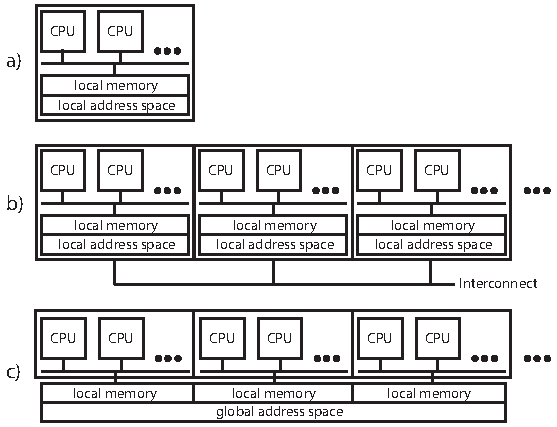
\includegraphics[width=1\textwidth]{Bilder/pgas.pdf}
	\caption{View on Shared Memory (a), Distributed Memory (b) and Partitioned Global Address Space (c)}
	\label{pgas_figure}
\end{figure}

Existing PGAS approaches are mainly comprised of dedicated programming languages such as Unified Parallel C (UPC) \cite{upc}, Co-Array Fortran \cite{co_array_fortran} or Chapel \cite{chapel} that allow for compiler optimizations in respect to distributed machines but lack portability and reach. In contrast to this, efforts exist to create libraries for existing programming languages used by many HPC systems.

\section{DASH C++ Template Library}
\label{dash_section}
DASH \cite{dash} is a compiler-free PGAS approach: It consists of a simple C++ library that can be compiled with any C++ compiler and thus can be used out-of-the-box on most HPC systems. The library is part of the Priority Programme ``Software for Exascale Computing'' (SPPEXA)\footnote[1]{\url{http://www.sppexa.de}} which supports research on computing systems achieving $10^{18}$ floating point operations per second and above. While PGAS languages require existing programs to be completely rewritten from scratch, DASH allows the applications to be incrementally ported and thus facilitates wider adoption of the PGAS model in the HPC community.

DASH operates on top of the \textit{DASH Runtime} (DART) which is a PGAS memory allocation and communication abstraction written in C. DART enables global memory allocation, pointers to remote memory locations and one-sided communication on top of existing libraries like MPI \cite{mpi3} or GASPI \cite{gaspi}. With DART-MPI \cite{dart_mpi}, a fully functional DART abstraction on top of MPI-3 is used in DASH releases at the time of this writing.

In DASH, processing elements are referred to as \textit{units}. Units can be any processing element such as threads or processes. DASH programs are implemented using the Single Program Multiple Data (SPMD) model: The data is partitioned onto the participating units and each unit executes the same code on its part of the data. Furthermore, units  form \textit{teams} that can be created at runtime. Because HPC hardware topologies become more complex over time (e.g. \cite{dragonfly}), DASH supports hierarchical team creation to allow for a more fine-grained exploitation of data locality compared to the typical local-remote distinction of the PGAS model.

Data is referred to in terms of global pointers and references. A \texttt{GlobPtr<T>} object holds information about the unit and local memory location of the referenced datum. It can be dereferenced to a \texttt{GlobRef<T>} object which behaves like a C++ reference and can be converted to an object of type \texttt{T}. This type conversion triggers a one-sided \texttt{get} operation transferring the data from its remote source to the caller. Similarly, data can be written into the referenced memory location of a \texttt{GlobRef<T>} object.

DASH provides a set of containers for distributed data storage. Aside from the static data structures Array and Matrix, dynamic data structures are available. Since the graph concepts of this work belong into the latter category, details of it are discussed in the following.\\

\subsection{Dynamic memory allocation}
\label{dash_mem_alloc_section}
Dynamic allocation in DASH is encapsulated in the \texttt{GlobHeapMem} concept. \texttt{GlobHeapMem} offers two basic operations to dynamically allocate memory during runtime: \texttt{grow} and \texttt{shrink}. These operations increase or decrease the local size of the memory allocated on the respective unit. Changes in memory space are not reflected in global address space until the operation \texttt{commit} is called which publishes the changes across all units.

A dynamic container in DASH pre-allocates some memory during its initialization. When the  memory is completely used, further additions of elements result in \texttt{GlobHeapMem.grow} operations. A call to the \texttt{barrier} operation of the container results in all newly added elements of the container to be publicly available on all units.\\

\begin{figure}[ht]
	\centering
  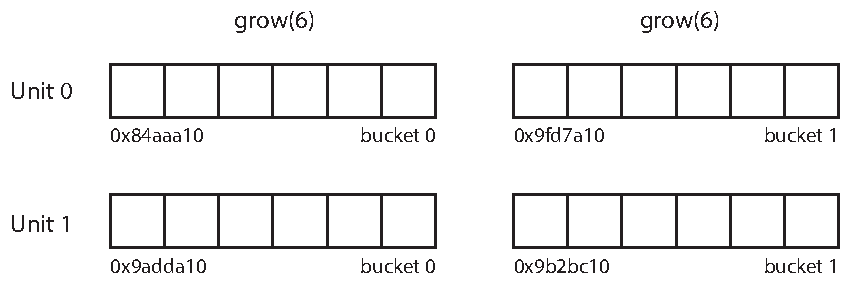
\includegraphics[width=1\textwidth]{Bilder/dash_dynamic_mem_space.pdf}
	\caption{Memory space of two units after two \texttt{GlobHeapMem.grow} operations}
	\label{dash_dynamic_mem_space_figure}
\end{figure}

Multiple \texttt{grow} operations result in a scattered memory space: Each call to \texttt{grow} creates a new \textit{bucket} - a contiguous memory region in the local freestore. A class implementing the \texttt{GlobHeapMem} concept keeps track of each bucket on each unit so that element indices can be translated to concrete memory locations. \autoref{dash_dynamic_mem_space_figure} illustrates the memory spaces of two units after two grow operations for six elements each have been called. The buckets are allocated at different memory locations. Data access to an element therefore requires the memory location of the bucket and the offset of the element inside the bucket. For this reason, bucket locations and sizes are exchanged between all units during a \texttt{commit} operation and a reference to the object holding the bucket data is needed in every iterator.

\chapter{Related work}
\label{related_work_section}
\section{Shared Memory}
Graph processing on distributed machines tends to result in low processor utilization due to bad locality \cite{graph_challenges}. Shared memory systems on the other hand allow for simpler graph algorithms with better processor utilization \cite{ligra}. Because some shared memory systems with several terabytes of memory exist (e.g. the LRZ teramem\footnote[1]{\url{https://www.lrz.de/services/compute/special\_systems/teramem/}}), graphs up to a certain size can also be computed on such systems. While many libraries and frameworks for graph processing on shared memory systems exist, this section only focuses on work relevant to the HPC community.\\

\textbf{Spatio-Temporal Interaction Networks and Graphs Extensible Representation (STINGER)} \cite{stinger} is a graph data structure for shared memory systems. STINGER tries to provide a standardized and extensible data structure that allows portability across different graph processing frameworks. The data structure consists of a set of standards that have to be abided by actual implementations.

At its core, STINGER is an adjacency list with a fixed structure. Vertices are stored in a contiguous memory region and point to blocks of edges. The set of all edges of a single vertex can be distributed between multiple blocks with each block containing a pointer to the next block. Vertices and edges both store a weight value and edges additionally store timestamps. This allows edges to be automatically removed after they have reached a certain age. STINGER also accounts for fault tolerance by defining standards for checkpointing functionality.\\

The \textbf{MultiThreaded Graph Library (MTGL)} \cite{mtgl} focuses on graph processing using specialized multithreading systems that contain processors supporting a large amount of thread contexts. The MTGL is specifically designed for the Cray MTA architecture which limits its use significantly because a Cray MTA system has to be available. Brian W. Barrett et al. have implemented an MTGL version for commodity hardware \cite{mainstream_mtgl} but its performance is significantly lower compared to the original version for serial machines.

The Cray MTA architecture \cite{tera_mta} utilizes processors with relatively slow speed and without data caches. Memory access is always blocking but each processor features a large amount of threads so that there are always free threads available for computation in most cases. This results in a simple and fine-grained synchronization model that is not available on commodity hardware, but also creates subtle concurrency and performance issues. These issues are addressed by the MTGL in order to allow straight-forward programming of graph algorithms on these platforms. 

Because of the architecture of the Cray MTA, locality is not an issue in the MTGL: Data is partitioned by the runtime system of the MTA. The interface of the MTGL is - like many graph processing frameworks - based on the Boost Graph Library (BGL) \cite{bgl}. It is less generic though: Only \textit{directed graphs} are supported and data is always stored in an \textit{adjacency list} structure.

\section{Distributed Memory}
Procession of large graphs that do not fit into the memory of a single machine takes place on distributed memory machines in HPC. Shared memory approaches that hold parts of the graph in persistent memory (e.g. GraphChi \cite{graphchi}) do not have sufficient performance in order to be useful in the field of high performance graph processing. However, because some graphs like scale-free social networks lack locality, graph partitioning on distributed memory machines is a challenge that can result in unpredictable performance due to low processor utilization \cite{mtgl}. While performance and scalability are key capabilities of the work mentioned in this section, they can not always be guaranteed.

\subsection{Bulk-synchronous graph processing}
\label{sync_graph_lib_section}
In \textit{Parallel Computing}, Valiant's \textit{Bulk Synchronous Parallel (BSP)} model \cite{bsp} describes a way to exploit locality: Data is partitioned across processors in a way that allows each processor to perform independent computations. BSP algorithms run a series of \textit{supersteps}, each consisting of three phases:

\begin{enumerate}
\item Local computation on each processor.
\item Global exchange of computed data between processors.
\item Synchronization of all processors.
\end{enumerate}

The performance of BSP algorithms relies heavily on a well-suited decomposition of the data. Because of the explicit barrier synchronization at the end of each superstep, processor time may be wasted on processors that finish their work faster than others. Deadlocks and data races are however prevented by it.\\

The \textit{Boost Graph Library (BGL)} \cite{bgl} is a widely used sequential graph processing framework. With the \textbf{Parallel Boost Graph Library (PBGL)} \cite{parallel_bgl}, the BGL has been ported to the environment of distributed machines using the BSP model. It aims at providing a general-purpose library for graph processing on distributed machines. The PBGL data structures adjacency list and adjacency matrix therefore are designed as generic as possible and the library includes a wide variety of different graph algorithms that can be extended with the \textit{Visitor Pattern} \cite{visitor_pattern}. Attributes of graph components are not restricted to simple edge weights: The PBGL allows programmers to define arbitrary attribute data structures for vertices and edges. Supported graph types in the PBGL include directed, undirected and bidirectional graphs.\\

\textbf{Pregel} \cite{pregel} is a framework for large-scale graph processing developed by Google. Like the PBGL, it partitions graphs by vertex and uses the BSP model for computation. Vertices are statically partitioned by a user-defined hash function. Pregel additionally accounts for fault tolerance with checkpointing mechanisms but only supports directed graphs. Programming in Pregel is restrictive because it only allows the definition of vertex visitors that have access to messages sent by other vertices in the previous superstep.

The static partitioning mechanism of Pregel can be replaced with a dynamic load balancing system called Mizan \cite{mizan}. It monitors Pregel graphs during runtime and migrates vertices to other partitions based on its observations.\\

\textbf{ScaleGraph} \cite{scalegraph2} is a graph processing library written in IBM's X10 \cite{x10} PGAS language. ScaleGraph supports graphs of arbitrary size. This means, it can also process graphs that do not fit completely into the memory of the used compute system. ScaleGraph supports dynamic graphs stored in an adjacency list data structure and static graphs stored in a sparse matrix data structure. For dynamic graphs, only directed edges are supported but ScaleGraph allows the programmer to define arbitrary attributes for vertices and edges. Because of bad performance experiences in the first version of the library \cite{scalegraph}, the garbage collection of X10 is disabled for big graphs. On top of the ScaleGraph core, Toyotaro Suzumura et al. have added an API based on the model of Pregel (see \autoref{sync_graph_lib_section}). Therefore, while the library is implemented using a PGAS language, it does not provide PGAS functionality to the user and rather relies on the BSP model of Pregel.

\subsection{Asynchronous graph processing}
The BSP model requires computation steps to be coarse-grained. This means that computations have to be performed on sufficiently large parts of the data that belong together to minimize costly communication. Some graphs however demand more fine-grained communication \cite{active_message_lib} which would require many BSP iterations with short computation steps resulting in low processor utilization. To account for these kind of graphs, algorithms that do not require explicit synchronization steps can be formulated to run asynchronously. Asynchronous execution of algorithms is especially useful in the field of machine learning \cite{graphlab}. Graph processing libraries have to explicitly support asynchronous communication because it requires atomic access to vertex and edge attributes.\\

Nicholas Edmonds et al. present a \textbf{graph processing library based on Active Messages} in \cite{active_message_lib}. It is based on the PBGL and tries to act as a next generation of the library. The library adds support for asynchronous active messages \cite{active_messages} that replace the two-sided communication used in the PBGL and transactions for access to graph component attributes. At the time of this writing, the library has not been released.\\

The \textbf{STAPL Parallel Graph Library (SGL)} \cite{stapl} is a PGAS library that aims at providing an API similar to sequential graph processing libraries. Thus, it tries to abstract data distribution by offering automated partitioning and load-balancing methods that achieve high scalability. Algorithms in the SGL can either be run bulk-synchronously or asynchronously. With an adjacency list data structure at its core, the SGL graph container is dynamic and a distributed directory is used to identify the location of vertices. This allows for the migration of vertices to other processors and redistribution schemes for load-balancing. The SGL is a promising approach in the field of PGAS graph processing libraries but as of this writing, no release or documentation is to be found.

\subsection{Linear algebra based graph processing}
Many graph algorithms can be expressed by a set of linear algebra operations \cite{fundamental_graph_alg}. The graph is represented by an adjacency matrix storing edge weights and additional vectors are used as auxiliary data structures. 

Because an adjacency matrix can be partitioned into blocks with each block being placed into the memory of a single processor, the graph can be partitioned in a 2-dimensional way. As research has shown, breadth-first-search and related algorithms can be implemented in a way that exploits the 2-D partitioning for higher performance in comparison to a 1-dimensional partitioning (i.e. partitioning based on vertices instead of edges) \cite{2d_bfs}.\\

The \textbf{Combinatorial BLAS} \cite{combinatorial_blas} exploits these findings with a library containing \textit{Basic Linear Algebra Subroutines} (BLAS) specifically targeted at graph processing. It provides a subset of typical BLAS operations like matrix-matrix multiplication that are sufficient for expressing most graph algorithms. Graph data is stored in a sparse matrix data structure. Vertices are therefore not mutable which results in graphs being static. Also, algorithms like Dijkstra's shortest path, that are based on priority queues, tend to have lower performance.\\

The Combinatorial BLAS is also used as a computational engine for a high-level graph processing framework: the \textbf{Knowledge Discovery Toolbox (KDT)} \cite{kdt}. The KDT aims at easing use of graph algorithms for domain experts that are not experts in computer science at the same time. To achieve this, it provides an API that allows to run algorithms on graphs with only few lines of code. Algorithm developers can extend the library by creating algorithms with the underlying linear algebra primitives. While KDT can be easily used by data scientists without background in computer sciences, the performance and scalability are still promising: In comparison to the PBGL, speedups from 3 to 12 for breadth-first search can be observed depending on the problem size and core count. Because it uses the Combinatorial BLAS as underlying engine, KDT also inherits its restrictions explained above.\\

For static graphs, \textbf{ScaleGraph} (see \autoref{sync_graph_lib_section}) also supports linear algebra primitives that can be used in the same way as with the Combinatorial BLAS.

\chapter{Graph container concepts}
\label{concept_section}
\section{Problem fundamentals}
A generic graph container must enable programmers to implement arbitrary graph algorithms with it. For this reason, an analysis of the problem domain is shown in this section. It results in functional requirements that are then used to deduce graph container concepts in later parts of this chapter.

\subsection{Elementary graph algorithms}
\label{graph_algo_section}
Most graph algorithms are based on two elementary graph algorithms: \textit{breadth-first search} and \textit{depth-first search} \cite{ita}. Support for these algorithms and any extensions to them therefore is an important requirement for a generic graph container. This section shortly describes both algorithms as well as selected algorithms extending them and analyses their requirements.

\subsubsection{Breadth-first search}
\textit{Breadth-first search (BFS)} finds all vertices reachable from a source vertex in a graph. The graph is traversed in a way that all vertices are found with the minimum number of edges connecting them to the source vertex: Starting from a certain vertex, all adjacent vertices are explored before their adjacent vertices are explored. All adjacent vertices of a given vertex are called \textit{frontier} or \textit{level}. BFS explores the vertices of a frontier and creates a new frontier for the next step that contains the adjacent vertices of the vertices in the current frontier.

\begin{lemma}
For successful graph traversal, adjacency information has to be accessible to any algorithm.
\end{lemma}

Because graphs tend to contain cycles, BFS employs a mechanism for already discovered vertices by graph coloring: All vertices start with a white color. As soon as a vertex is discovered for the first time, its color is changed to grey. Its color is changed to black once all of its adjacent vertices have been discovered. This results in the frontier being colored grey and all other processed vertices being colored black so that the traversal can be progressed in a breadth-first manner.

BFS can be used to construct a \textit{breadth-first tree} that contains all paths from the source vertex to its reachable vertices.

\begin{lemma}
For BFS to work, a graph container must be able to store mutable attributes for vertices: color and predecessor. A breadth-first tree might be later extracted from the predecessor attributes but it can be convenient if the graph container allows the tree to be constructed in an external data structure during computation of the algorithm. 
\end{lemma}

\begin{lemma}
Frontiers need to be managed with a queue or a similar data structure. This data structure might be external or part of the graph container itself. For distributed environments, the vertices of the frontier must be distributed to the nodes holding the respective vertices. The queue data structure therefore has to be distributed.
\end{lemma}

Because BFS naturally finds the paths with the least edges between vertices, it is obvious that it can be used for \textit{shortest path computation}. \textbf{Dijkstra's shortest path algorithm} \cite{dijkstra} for example is an extension to BFS: Each edge is associated with a distance attribute. Progressing in a breadth-first manner, the smallest sum of edge distances is saved in vertices as an additional attribute. If a vertex is discovered from an edge with a smaller distance sum, the attribute's content is replaced with this new sum.

Similar to Dijkstra's shortest path algorithm, a minimum spanning tree algorithm such as \textbf{Prim's algorithm} \cite{prim} traverses a graph in breadth-first order and creates a tree based on the minimum of edge weight attributes for each frontier.

\begin{lemma}
Graph containers do not only have to support vertex attributes. Edge attributes are also relevant. While Dijsktra's shortest path algorithm only requires a single attribute for edges, other algorithms might require more.
\end{lemma}

\subsubsection{Depth-first search}
\textit{Depth-first search (DFS)} explores vertices starting from a source vertex just like BFS. It differentiates from BFS in that it processes vertices in another order: Instead of exploring the vertices of a frontier one after another, DFS explores adjacent vertices directly from the most recently discovered vertex. If all adjacent vertices have been completely explored, DFS uses backtracking, i.e. it returns to the vertex from which the current vertex has been explored, and progresses there. Once finished, DFS proceeds to start another iteration from an arbitrary vertex that has not been discovered in the first iteration - contrary to BFS.

DFS uses a graph coloring scheme similar to BFS. Vertices visited for the first time are colored grey and when the backtracking takes effect, the respective vertex is colored black meaning that all edges from this vertex have been explored. DFS does not need a supporting data structure but apart from that has the same requirements on graph containers as BFS.

Some algorithms use DFS as a subroutine. For example, a \textbf{topological sort} of a graph runs DFS and then creates a list with sorted vertices based on the findings of the DFS subroutine. A \textbf{strongly connected components} algorithm runs DFS on the graph and then on the transposed version of the graph (i.e. the graph with reversed edges).

\begin{lemma}
Some algorithms have to access graph attributes after another algorithm has stored them inside the graph. For this reason, attributes of all vertices and edges have to be persistent and accessible across single algorithms.
\end{lemma}

Because BFS and DFS traverse a graph in such a fundamentally different way, it becomes obvious why locality is problematic with distributed graphs: If a graph partitioning results in high locality exploitation for BFS, it will result in low locality exploitation for DFS and vice versa.

\begin{lemma}
Partitioning of distributed graphs is dependent on locality information in the graph data itself and the algorithm used. Therefore, no generally valid partitioning scheme can be employed and locality information about a graph as well as information about the used algorithms is needed in advance for a reasonable partitioning.
\end{lemma}
 

\subsection{Functional requirements}
Based on the observations of \autoref{graph_algo_section}, the following functional requirements for a PGAS graph abstraction have been deduced:

\begin{tabularx}{1\textwidth}{| X | X |}
  \hline
  \textbf{Requirement} & \textbf{Notes} \\ 
  \endhead  
  \hline
  Vertex element creation & Creation of single vertices inside the graph data structure \\ \hline
  Edge element creation & Creation of single directed or undirected edges inside the graph data structure \\ \hline
  Vertex element deletion & Removal of single vertices from the graph data structure \\ \hline
  Edge element deletion & Removal of single edges from the graph data structure \\ \hline
  Global element iteration & Iteration over vertices, edges and adjacent vertices of the whole data structure \\ \hline
  Local element iteration & Iteration over vertices, edges and adjacent vertices of parts of the data structure hosted on the same machine \\ \hline
  Vertex attribute creation & Permanent storage of attributes belonging to particular vertices along with these vertices \\ \hline
  Edge attribute creation & Permanent storage of attributes belonging to particular edges along with these edges \\ \hline
  Vertex attribute mutation & Adjustment of attributes belonging to particular vertices \\ \hline
  Edge attribute mutation & Adjustment of attributes belonging to particular edges \\ \hline
  Global, asynchronous element access & Access to elements on other machines without synchronization enforcement \\ \hline
  Global, asynchronous attribute access & Access to attributes belonging to particular elements on other machines without synchronization enforcement \\ \hline
  User-specified data distribution & Storage location of elements and attributes specified by the user \\ \hline
  Global dynamic memory allocation & Allocation of memory for elements and attributes across multiple machines during runtime \\ \hline
  Global dynamic memory de-allocation & Freeing of memory for elements and attributes across multiple machines during runtime \\ \hline
  Epoch-based memory space synchronization & Explicit synchronization of newly added/removed memory space between machines in user-defined time-steps \\ \hline
  Container meta-data retrieval & Retrieval of container meta-data like \textbf{number of vertices} during runtime \\ \hline
\end{tabularx}

\section{Container concepts}
This section describes graph container concepts that have been deduced from the related work analysis of \autoref{related_work_section} and the graph algorithm analysis of \autoref{graph_algo_section}. The concepts follow the C++ standard library's container concept schemes. A complete concept definition can be found in \autoref{concept_appendix}.

\begin{figure}[ht]
	\centering
  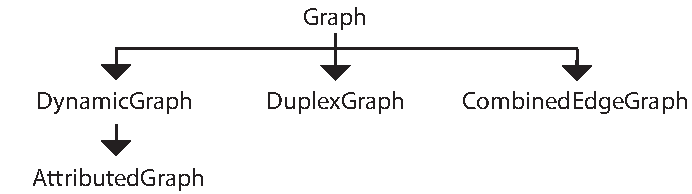
\includegraphics[width=0.8\textwidth]{Bilder/concepts.pdf}
	\caption{Hierarchy of graph container concepts}
	\label{concepts_figure}
\end{figure}

\autoref{concepts_figure} depicts the different concepts and their relationships to each other. The \texttt{Graph} concept provides basic functionality for graph processing while the other concepts refine it with additional functionality.

\subsection{Graph}
The \texttt{Graph} concept describes a graph container for static data that is suitable for \textit{directed graphs}. It consists of a constructor that creates a graph based on an existing \textit{edge list}.

The constructor takes two iterators of type \texttt{InputIterator} which allows the edge list to be of any STL-compatible container type (e.g. \texttt{std::list}). An edge list has  to contain elements of type \texttt{std::pair} with both contained types being integers describing unique vertices. The constructor then creates the graph by adding vertices based on these integers and connecting them according to the given vertex pairs.

Vertices and edges are represented by their own types. Edge types have to contain data identifying the source and target vertices. Since the \texttt{Graph} concept does not comprise an index space, iterators may be used for this task depending on their implementation. The concept is however compatible to index spaces being implemented on top of it.

Vertices and edges are assigned to the local memory of a node if the corresponding edge list has been assigned to the constructor of this node. Nodes can then iterate over elements either locally (over the elements that directly reside in the node's memory) or globally (over all elements in the graph) by calling the respective iterators. Due to the default \texttt{Graph} concept describing a static graph, no more elements can be added or removed after the constructor has been called.

The \texttt{Graph} concept contains two kinds of iterators:

\begin{itemize}
\item Vertex iterators
\item Out-edge iterators
\end{itemize}

This is the minimum needed for adjacency iteration: Each node can iterate over the set of all vertices or its local portion of the vertices and for each vertex, the outgoing edges can be iterated. Global iterators should facilitate a mechanism for direct local dereferencing if the respective element resides on the local machine of the calling node. 

\autoref{adj_it_code} shows an adjacency iteration over all outgoing edges of local vertices. Since all edges belonging to a particular vertex reside on the same node, only local iterators are available for adjacency iteration of a given vertex identified by a local iterator (\texttt{it}).

\begin{lstlisting}[caption=Adjacency iteration with Graph concept\label{adj_it_code}] 
std::list<std::pair<int, int>> edge_list = { {1, 2}, {1, 3}, {4, 1} };
Graph g(4, 3, edge_list.begin(), edge_list.end());

for(auto v_it = g.vertices().lbegin(); v_it != g.vertices().lend(); ++v_it) {
  for(auto e_it = g[v_it].out_edges().lbegin(); e_it != g[v_it].out_edges().lend(); ++e_it) {
    Graph::edge_type e = *e_it;
  }
}
\end{lstlisting}

\subsection{DynamicGraph}
The \texttt{DynamicGraph} concept extends the \texttt{Graph} concept with functionality for dynamic addition and deletion of graph elements during runtime. Because elements can be added after construction of the graph, an upfront initialization with an edge list is not required here. For this reason, a new constructor allows the graph to be created without any elements. It initializes the graph with a certain capacity so that each node has a fixed part of memory already assigned to it. Contrary to the constructor of \texttt{Graph}, the number of edges is not an absolute number but rather the number of edges per vertex. This means that the reserved capacity for edges equals to $number of vertices * number of edges$. The vertex and edge numbers are supplied for the whole graph, meaning that they have to be multiples of the amount of nodes participating in the memory allocation for the container.

All methods for adding and removing vertices and edges can be called with either local or global iterators pointing to them. 

Dynamic data changes of the graph are not reflected in global memory space until the user explicitly issues a \texttt{commit} operation. Before that, the changes can only be seen on the same node using local iterators. A \texttt{commit} operation can invalidate global iterators.

Creation and deletion of elements happens locally on each node. The resulting changes in 
local memory and iteration space are not reflected in the respective global spaces until the graph's \textit{barrier synchronization} is called. This \textit{epoch-based} synchronization allows for a trade-off between dynamics and performance.

\autoref{dynamic_graph_code} shows an empty graph being constructed and two vertices and an edge between them being added to it.

\begin{lstlisting}[caption=Dynamic creation of graph elements\label{dynamic_graph_code}] 
DynamicGraph g(4, 3); // creates a graph with 0 elements but capacity for
                        // 4 vertices and 12 edges

auto v1 = g.add_vertex(); // returns index of created vertex
auto v2 = g.add_vertex();

auto e1 = g.add_edge(v1, v2);

g.commit();               // changes are published
\end{lstlisting}

\subsection{AttributedGraph}
The \texttt{AttributedGraph} concept extends the \texttt{Graph} concept with attributed elements. The user can specify static structs (a struct in a contiguous memory region without pointers and references) for vertices and edges respectively. A constructor allows concrete instances of these structs to be added to each element. Vertex and edge types contain copies of the struct instances and make them publicly available. Attributes can be replaced.

\autoref{attributed_graph_code} shows a graph being constructed with two vertices and an edge between them. The vertices and edges store an attribute \textit{id}.

\begin{lstlisting}[caption=Graph construction with attributed elements\label{attributed_graph_code}] 
typedef   std::tuple<
    std::pair<int, v_prop>,
    std::pair<int, v_prop>,
    e_prop
> tuple_t;

struct v_prop {
  int id
};

struct e_prop {
  int id
};

v_prop vp1 { 1 };
v_prop vp1 { 2 };
v_prop ep1 { 1 };
tuple_t e1 = std::make_tuple(
  std::make_pair(1, vp1),
  std::make_pair(2, vp2),
  ep1
);

std::list<tuple_t> edge_list = { e1 };
AttributedGraph<v_prop, e_prop> g(2, 1, edge_list.begin(), edge_list.end());
\end{lstlisting}

A \texttt{DynamicGraph} that also satisfies the requirements of \texttt{AttributedGraph} can add attributes on-the-fly, reducing the complexity of the syntax. An example is shown in \autoref{dynamic_attributed_graph_code}.

\begin{lstlisting}[caption=Dynamic creation of attributed graph elements\label{dynamic_attributed_graph_code}] 
struct v_prop {
  int id
};

struct e_prop {
  int id
};

AttributedDynamicGraph<v_prop, e_prop> g(2, 1);
v_prop vp1 { 1 };
auto v1 = g.add_vertex();
g.set_attribute(v1, vp1);
v_prop vp2 { 2 };
auto v2 = g.add_vertex();
g.set_attribute(v1, vp1);
e_prop ep1 { 1 };
auto e1 = g.add_edge(v1, v2);
g.set_attribute(e1, ep1);
g.commit();
\end{lstlisting}

\subsection{DuplexGraph}
\label{duplex_graph_section}
The \texttt{DuplexGraph} concept extends the \texttt{Graph} concept with iterators for inbound edges. It is a requirement for \textit{undirected} and \textit{bidirectional graphs} and optional for \textit{directed graphs}.

\autoref{duplex_code} shows a graph with two edges pointing from \textit{vertex 1}. These edges are then iterated with the inbound edge iterator.

\begin{lstlisting}[caption=Inbound edge iteration\label{duplex_code}] 
std::list<std::pair<int, int>> edge_list = { {1, 2}, {1, 3}, {4, 1} };
Graph g(4, 3, edge_list.begin(), edge_list.end());

auto v_it = g.vertices().lbegin();

for(auto e_it = g[v_it].in_edges().begin(); e_it != g[v_it].in_edges().end(); ++e_it) {
  Graph::edge_type e = *e_it; // returns edge (4, 1)
}
\end{lstlisting}

\subsection{CombinedEdgeGraph}
The \texttt{CombinedGraph} concept extends the \texttt{Graph} concept with iterators for a combination of inbound and outbound edges. It is advised that an implementation also satisfies \texttt{DuplexGraph}, but this is not a requirement. The specific iteration order for the combination of inbound and outbound edges is not specified in this concept. It is left to the implementation.

\begin{lstlisting}[caption=Combined edge iteration\label{combined_edge_code}] 
std::list<std::pair<int, int>> edge_list = { {1, 2}, {1, 3}, {4, 1} };
Graph g(4, 3, edge_list.begin(), edge_list.end());

auto v_it = g.vertices().lbegin();

for(auto e_it = g[v_it].edges().begin(); e_it != g[v_it].edges().begin(); ++e_it) {
  Graph::edge_type e = *e_it; // returns edges (1, 2), (1, 3) and (4, 1)
}
\end{lstlisting}

\section{Memory spaces}
\label{memspace_section}
A \texttt{Graph} contains two distinct memory spaces for vertices and outbound edges. A \texttt{DuplexGraph} additionally contains a memory space for inbound edges. Each memory space comprises its own iteration space (see \autoref{iteration_concept_section}). Memory spaces are maintained on a per-node basis and new memory is allocated locally with an STL-compatible container. The concrete container implementation can be specified by the user but it must allocate \textit {contiguous memory regions} (note: in C++17 \cite{c++17}, this means the container must satisfy the requirements of the \texttt{ContiguousContainer} concept. Because this work is based on C++11, no formal requirement can be formulated). By default, \texttt{std::vector} should be used as allocator.

An object maintaining a memory space on a certain node also holds information about the memory spaces on all other nodes. Changes in local memory space are hidden from other nodes until a \texttt{commit} operation initiates a communication step that exchanges information about the occupied memory.

Remote data can then be accessed with this information using \textit{Remote Direct Memory Access (RDMA)} features of the used communication layer (e.g. MPI-3).\\

The concrete memory model is up to the implementation. The publicly visible memory space however has to adhere to the following definitions:

\begin{defi}
Local vertex memory space is logically contiguous. New elements are either added at the end of the memory space or, if available, at the position of elements marked for deletion.
\end{defi}

\begin{defi}
Local edge memory space consists of multiple logically contiguous edge-list memory spaces that are connected to each other in arbitrary order.  New elements are either added at the end of their respective edge-list memory spaces or, if available, at the position of elements marked for deletion in their respective edge-list memory spaces.
\end{defi}

\begin{defi}
Global memory spaces are a union of local memory spaces ordered by their node ID ascendingly.
\end{defi}

Memory spaces do not have to be completely contiguous in memory. They can consist of several contiguous memory regions. For each of these memory regions, the beginning memory address as well as the length has to be stored. An abstraction can then use this information to present a contiguous memory region to the public.

\autoref{memspace_figure} shows exemplary logical memory spaces for vertices and edges respectively. The memory spaces appear contiguous to the outside but parts of them might reside in different memory locations depending on the implementation.

\begin{figure}[ht]
	\centering
  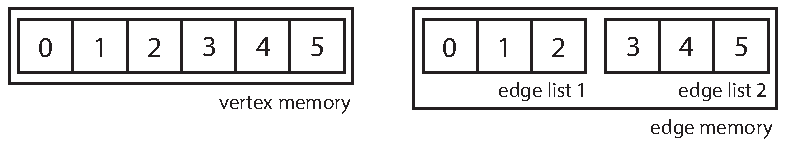
\includegraphics[width=1\textwidth]{Bilder/memspace.pdf}
	\caption{Vertex and edge memory space abstractions}
	\label{memspace_figure}
\end{figure}

\section{Iteration spaces}
\label{iteration_concept_section}
Elements in all graph concepts of this work are identified by iterators. Two different kinds of iterators exist:\\

\textbf{Global iterators} identify elements in the whole graph. They are needed to iterate over portions of the graph that do not reside locally on a node and to access these elements. Dereferencing a global iterator yields a global reference which in turn can be dereferenced to access the actual data. A \textit{global reference} is therefore responsible for \textit{remote memory access}.\\

\textbf{Local iterators} identify elements residing locally on a node. A simple pointer to a contiguous memory region can already suffice for this task. However, dynamic containers usually require multiple memory regions to be created during their lifetime. Because local iterators must be able to iterate over the complete local portion of the elements, a more sophisticated abstraction will be needed in case the local memory space consists of more than one contiguous region.\\

Global and local iterators have to strictly follow the \texttt{STL Iterator} concepts in order to be usable by STL algorithms. Additionally, they have to implement mechanisms geared towards PGAS concepts. For example, a global iterator should provide a possibility for finding out if the element it points to resides locally or on a remote node. This work is based upon \texttt{DASH Iterator} concepts \cite{dash_new} that are suitable for any implementation of the presented graph concepts.\\

Global and local iteration spaces directly map to global and local memory spaces explained in \autoref{memspace_section}. Because of this, iterators are invalidated when changes to the memory spaces are published.

\section{Index spaces}
\label{indexspace_section}
The concepts of this work do not comprise index spaces. They can however be implemented on top of them and exist alongside the iteration spaces that are primarily used to identify elements. This section gives a brief overview of possibilities in this regard:\\

Simple integer index spaces like they are used in STL containers (e.g. \texttt{std::vector}) or static DASH containers (e.g. \texttt{dash::Array}) are problematic: Because element creation in dynamic containers requires new indices to be generated during runtime, all nodes would have to find consensus so that index numbers are continuous and unique. This would require one of the following mechanisms:

\begin{enumerate}
\item Increment a global \textit{maximum index number} on each element creation.
\item Create a local index on each element creation and negotiate global indices for multiple elements during \texttt{commit} operations.
\end{enumerate}

\textit{Variant 1} requires communication between nodes every time an element is created. This additional overhead is intolerable for high performance applications and therefore not suitable for this concept.\\

\textit{Variant 2} only adds communication during the \texttt{commit} operation. If new elements have been created, the \texttt{commit} operation executes all-to-all communication. An additional mechanism that negotiates index numbers could therefore be performed in the same communication steps adding only a slight overhead. Unfortunately, using the created elements locally before a \texttt{commit} requires the user to handle the elements with a temporary local index that is later substituted by a global index. This leads to additional programming complexity.\\

A split index can be used to circumvent this problem:

\begin{enumerate}\addtocounter{enumi}{2}
\item Use indices with multiple components (global and local).
\end{enumerate}

\textit{Variant 3} allows for indices to be created without global consensus: Indices contain the node ID and the local index on that node. This however comes with another problem: If mechanisms for element migration are employed, the global (node) part of the indices has to be either changed or a global directory structure has to be built in order to redirect requests of a certain index to the correct node.

\chapter{Reference implementation}
\label{impl_section}
This section explains a concrete reference implementation of the concepts in \autoref{concept_section}. The implementation is part of the DASH C++ Template Library and thus written in C++11. It is based on basic C++ concepts illustrated in \autoref{cpp_section}. The reference implementation will be referred to as \texttt{dash::Graph} in this chapter.

\section{Overview}
\texttt{dash::Graph} is part of the dynamic data containers of the DASH Library. As such, it is interacting with existing components of the library. \autoref{impl_overview_figure} depicts the components and their main interactions.\\

\begin{figure}[ht]
	\centering
  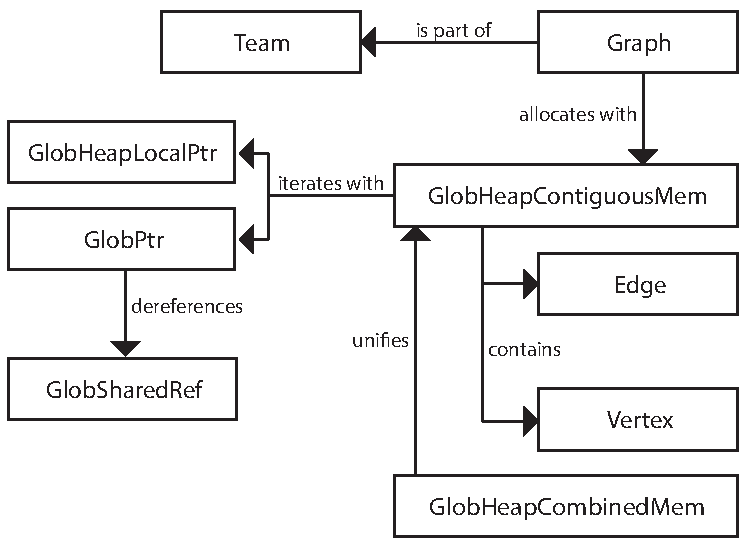
\includegraphics[width=0.9\textwidth]{Bilder/impl_overview.pdf}
	\caption{dash::Graph component overview}
	\label{impl_overview_figure}
\end{figure}

The \texttt{Graph} gets initialized with a reference to an existing \texttt{Team}. By default, this is \texttt{Team::All()} which includes all units (see \autoref{dash_section}) DASH has been initialized with. The \texttt{Graph} creates three instances of \texttt{GlobHeapContiguousMem} for vertices, inbound edges and outbound edges. These instances are used to globally allocate memory for the respective elements. Since the \texttt{Graph} also allows for the iteration of all (inbound and outbound) edges, \texttt{GlobHeapCombinedMem} unifies the memory spaces of the two \texttt{GlobHeapContiguousMem} instances. Both \texttt{GlobHeapContiguousMem} and \texttt{GlobHeapCombinedMem} use a specialized template version of \texttt{GlobPtr} to iterate over the memory space. Each \texttt{GlobPtr} object can then be dereferenced to a \texttt{GlobSharedRef} object which enables remote memory access to the referenced element. For locally residing elements, \texttt{GlobPtr} dereferences to a local reference pointing to a concrete memory location.

\subsection{Data structure}
The reference implementation's underlying data structure is an \textit{adjacency list}. It consists of a logically contiguous array of vertices and two logically contiguous arrays of edges (inbound and outbound edges respectively). The arrays are connected with each other by a separate data structure that stores information about starting point and length of an edge list belonging to a particular vertex. \autoref{data_structure_mapping_figure} depicts the mapping of vertices to their corresponding edge lists.

\begin{figure}[ht]
	\centering
  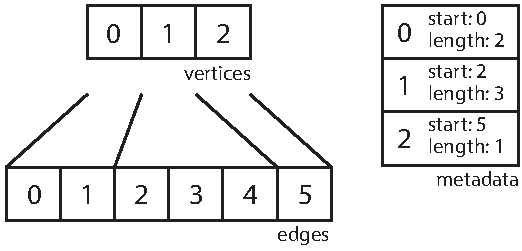
\includegraphics[width=0.7\textwidth]{Bilder/data_structure_mapping.pdf}
	\caption{Data structure mapping}
	\label{data_structure_mapping_figure}
\end{figure}

Vertices and edges are modeled as individual classes: \texttt{Vertex} and \texttt{Edge}.Because the meta-information that links the vertex array to the edge arrays is also used by iterators it is not stored inside of the \texttt{Vertex} objects but in an independent data structure. Vertices store attribute information only, while edges additionally store identifiers of their source and target vertices. While \texttt{dash::Graph} exposes only iterators to the public, source and target vertices are identified by indices internally because iterators can be invalidated during \texttt{commit} operations and because the iterators in use have a higher memory consumption.

Attribute information can only consist of variables of static size. These variables are filled with default values upon initialization as per \textit{default initialization} of the C++ standard.

\subsection{Pointers and references}
To allow \texttt{GlobPtr} and \texttt{GlobSharedRef} act like real pointers and references respectively, operators like the increment and dereference operators are overloaded. This results in usage analogous to native pointers and references:

\begin{lstlisting}[caption={Operator overloading in GlobPtr and GlobSharedRef}\label{globptr_code}] 
typedef GlobHeapContigousMem<std::vector<int>> g_mem_type;
GlobPtr<int, g_mem_type> ptr(mem, 0);     // position 0 in index space
++ptr;                                    // go to position 1 in index space
auto ref = *ptr;                          // dereference ptr to GlobSharedRef object
int val = ref;                            // convert reference to value
\end{lstlisting}

In this case, \texttt{mem} is an instance of \texttt{GlobHeapContiguousMem} holding at least two globally available elements.

\subsection{Graph types}
\label{graph_types_section}
\texttt{dash::Graph} currently supports \textit{directed} and \textit{undirected} graph types. A bidirectional graph type is not implemented but is consistent with the graph concept and can therefore be integrated. As described in \autoref{duplex_graph_section}, directed graphs can be instantiated in two different variants depending on the need for inbound edge iteration. This is due to the fact that this iteration method is not necessary for some algorithms and requires additional communication that lowers the overall performance of the graph, even if not used at all.

For undirected graphs, edges are replicated to the edge lists of both participating vertices. For directed graphs, the same mechanism is used when inbound edge iteration is needed. Edges in directed graphs without inbound edge iteration are not replicated in any way.

\section{Memory management}
\label{mem_mgmt_section}
\texttt{dash::Graph}'s memory space is handled by \texttt{GlobHeapContiguousMem}. This class follows the concept described in \autoref{memspace_section} but adds an additional feature: Fully contiguous global memory regions. While the memory concept only demands single edge lists to be contiguous, \texttt{GlobHeapContiguousMem} allocates a contiguous memory space for all globally visible vertices and edges for better locality exploitation. However, this comes at the expense of additional memory re-allocations in each epoch.

\subsection{Contiguous memory}
\label{contiguous_mem_section}
\autoref{contiguous_mem_figure} illustrates the basic scheme of the contiguous memory allocation. \textit{Region 1} is a publicly available contiguous memory region. The memory location of \textit{region 1} is known by other units and thus cannot be changed outside of a commit operation. Because of this, \textit{region 2} is allocated at another memory location that might not be contiguous to \textit{region 1}. \textit{Region 2} contains elements that have been added in the current epoch - they are available only locally and cannot be seen by other units.

The \texttt{commit} operation starts a new epoch by packing the elements of the two memory regions into another contiguous memory region and notifying other units about the changed location and size of the region. Traversing the elements in this region is now as simple as incrementing a pointer. Local iteration over the elements however requires a hop between the publicly available region and the local-only region because they are not contiguous. \texttt{GlobHeapLocalPtr} can iterate over an arbitrary number of buckets with contiguous memory (see \autoref{iteration_impl_section}). In this case, always two buckets (the two mentioned memory regions) are used.

\begin{figure}[ht]
	\centering
  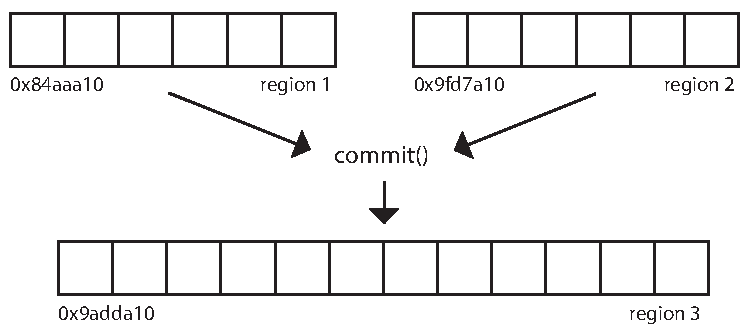
\includegraphics[width=0.9\textwidth]{Bilder/contiguous_mem.pdf}
	\caption{Contiguous memory allocation}
	\label{contiguous_mem_figure}
\end{figure}

\subsection{Edge list memory}
Each edge list has to be maintained with individual second regions for element insertions: The mechanism in \autoref{contiguous_mem_section} is used for each edge list individually and the \texttt{commit} operation packs all edge lists into one contiguous memory region.\\

\subsection{Element deletion}
Element deletion is not implemented at the time of this writing. This section however describes how a deletion mechanism can be implemented.

Deleting an element in contiguous memory regions requires its memory location to get invalidated instead of removed to avoid shifting of elements and offset invalidation. If many delete operations occur, the memory space will get scattered. For this reason, it is necessary to take measures that reduce the scattering of the memory to a minimum. A \textit{free list} is a simple way to achieve this: Deleting an element results in its memory location being added to the free list. If another element is added, a memory location from the back of the free list is used to store the element. Only if the free list is empty, new memory is allocated.

Because invalidated elements are not part of the memory space anymore, iterators must have access to the free list so that they can skip the respective elements.

\section{Iteration}
\label{iteration_impl_section}
The four different iteration spaces of the graph concept (see \autoref{iteration_concept_section}) are handled by the same iterator classes. Since the memory space of \texttt{dash::Graph} is epoch-based, iteration space of local iterators can be different to the local part of the iteration space of global iterators.

\subsection{Local iteration}
\label{local_iter_section}
Local iteration in dynamic containers of DASH is handled by \texttt{GlobHeapLocalPtr} that can iterate over multiple non-contiguous memory buckets. \texttt{GlobHeapContiguousMem} holds a list of objects containing bucket meta-data including size and a local native pointer to its beginning memory location. The bucket list is passed to a \texttt{GlobHeapLocalPtr} along with the position the pointer currently holds in the index space of the buckets. The buckets are equal to the allocated memory regions of \texttt{GlobHeapContiguousMem} as described in \autoref{mem_mgmt_section}.

Iteration is done by \texttt{increment}/\texttt{decrement} operations which result in \texttt{GlobHeapLocalPtr} calculating the bucket number the current position belongs to. A \texttt{dereference} operation then accesses the local pointer of the bucket object.

\subsection{Global iteration}
\label{global_iter_section}
For global iteration, a template specialization of \texttt{GlobPtr} for \texttt{GlobHeapContiguousMem} is used. It is similar to the template specialization of \texttt{GlobPtr} for \texttt{GlobHeapMem}, which is used for other dynamic DASH containers like \texttt{dash::List}.

While the bucket meta-data used by \texttt{GlobHeapLocalPtr} contains only information about local buckets, \texttt{GlobPtr} requires information about all buckets on all units. Therefore, \texttt{GlobHeapContiguousMem} distributes bucket information between all units during a \texttt{commit} operation. This information includes bucket sizes as well as DART global pointers to the memory locations of the buckets in global address space.

With the bucket size information and the DART abstraction of global pointers, \texttt{GlobPtr} can iterate over global memory space the same way as \texttt{GlobHeapLocalPtr} iterates over local memory space. The iteration order is given by the canonical order of units.

\subsection{Edge iteration}
Inbound and outbound edges are handled by separate \texttt{GlobHeapContiguousMem} objects. Iteration of either is therefore handled as described in \autoref{local_iter_section} and \autoref{global_iter_section}. The \texttt{CombinedEdgeGraph} concept however requires iteration over all existing edges. For this reason, \texttt{GlobHeapCombinedMem} is used to unify the iteration spaces of multiple \texttt{GlobHeapContiguousMem} objects.

\begin{figure}[ht]
	\centering
  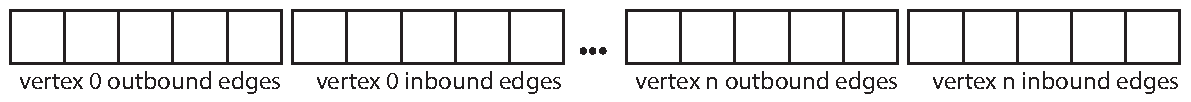
\includegraphics[width=1\textwidth]{Bilder/combined_edges.pdf}
	\caption{Combined edge iteration space}
	\label{combined_edges_figure}
\end{figure}

\autoref{combined_edges_figure} illustrates the order in which the combination of inbound and outbound edges are iterated over.

\section{Data access}
Remote memory data access is strictly handled via \texttt{GlobSharedRef} objects. These objects issue DART \texttt{get}/\texttt{put} operations to access data on remote machines. If referenced data resides locally, \texttt{GlobSharedRef} directly accesses it in the memory.

Because edges are replicated for some graph types (see \autoref{graph_types_section}), writing data to an element with a \texttt{GlobSharedRef} object would introduce consistency problems as it is restricted to referencing single memory locations. At the time of this writing, the reference implementation does not support a mechanism to cover this problem. It can however be achieved by another kind of \textit{global reference} that additionally stores locations of replicated edges.

\chapter{Case studies}
\label{case_studies_section}
This chapter illustrates use cases for the previously described graph concepts using the reference implementation explained in \autoref{impl_section}. These use cases are then evaluated against existing implementations in \autoref{eval_section}.

The use cases consist of two important basic graph algorithms: \textit{connected components} and \textit{minimum spanning tree}. Both algorithms have been examined in PGAS implementations using the UPC programming language \cite{upc} and their implementations in this work will roughly follow the specifications explained in \cite{pgas_algorithms} which consists of shared-memory algorithms ported to UPC.

\section{Optimizations}
While shared-memory algorithms can be directly ported to distributed machines in PGAS, performance might suffer from irregular data accesses across machines as the latency of the network is much higher than the latency of memory access in shared-memory machines. Cong et al. therefore propose performance optimizations including \textit{communication coalescing} and \textit{cache performance optimization}. While the results show that these optimizations are significant (up to 5 times faster for the designated graph size), this case study only employs the \textit{communication coalescing} optimization because it is the most beneficial for scalability and an implementation of all optimization techniques is beyond the scope of this thesis.

\subsection{Communication coalescing}
\label{comm_coal_section}
Because shared-memory algorithms typically do not employ domain decomposition the way needed for distributed systems, processors issue many access requests to data belonging to other processors. On a shared-memory system, this is not problematic as the access latency is the same or, in case of NUMA domains, only slightly higher. On distributed systems however, these accesses result in remote memory accesses for which the latency is determined by the network and therefore orders of magnitude higher. Thus, directly porting shared-memory algorithms in the PGAS space can result in low performance.

To overcome this problem, data accesses have to happen in batches rather than individually (similar to bulk-synchronous messaging in BSP models). The \textit{communication coalescing} mechanism of \cite{pgas_algorithms} proposes to collect all data reads and/or data writes of one synchronization step and distribute them to the respective processors in one message. In \autoref{comm_coal_algorithm}, a less generalized version of the algorithm that does not account for local cache-performance optimization is shown.\\

\begin{center}
\begin{algorithm}[h]
 \KwData{array \textit{indices} of indices to read}
 \KwResult{array \textit{output}}
 sort \textit{indices} by processor ID and save permutations\;
 alltoall(\textit{indices}, \textit{indices\_recv})\;
 \For{$i \gets 0$ \textbf{to} $indices\_recv.size()$} {
   \textit{data}[i] $\gets$ data attribute of the element $indices\_recv$[i]\;
 }
 alltoall(\textit{data}, \textit{data\_recv})\;
 restore original order with saved permutations on \textit{data\_recv}\;
 return \textit{data\_recv}\;
 \caption{Communication coalescing algorithm for data reads}
 \label{comm_coal_algorithm}
\end{algorithm}
\end{center}

A \textit{communication coalescing} algorithm for data writes works analogously.

\section{Graph algorithms}
This section presents a description of the algorithms used in the case studies as well as a high level description of their implementation.

\subsection{Connected Components}
\textit{Connected components} is an elementary graph algorithm based on depth-first-search \cite{ita}. It aims to find components in a graph in which every vertex is connected to at least one other vertex. The algorithm finds one or more sub-graphs with no edges between them. \autoref{cc_figure} depicts a graph comprising two connected components.

\begin{figure}[ht]
	\centering
  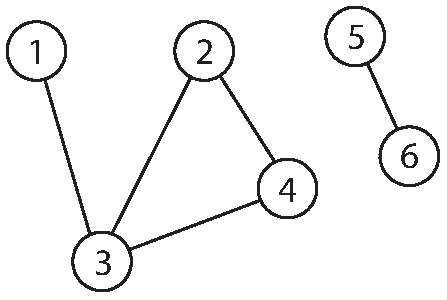
\includegraphics[width=0.5\textwidth]{Bilder/cc.pdf}
	\caption{Graph with two connected components}
	\label{cc_figure}
\end{figure}

The classical variant of the algorithm performs a depth-first search on a graph $G$ and another depth-first search on the transposed version of the graph $G^T$.
Because locality can hardly be exploited in depth-first search and because two runs per iteration are necessary to compute this algorithm, variations of the algorithm exist that account for better performance \cite{lineartime_cc} \cite{simple_cc}. 

The algorithm used in this case study is based on the shared-memory version found in \cite{pgas_algorithms}. Contrary to the classical variant of the algorithm, no depth-first search is performed. All edges of the graph are examined in an arbitrary order leading to much better locality exploitation: Each processor can examine the edges in the order they are placed in memory.

The algorithm requires vertex attributes for the parent component a vertex belongs to. This parent component attribute is initially set to the vertex itself. The algorithm then proceeds with iteration over the following two steps until no more component changes can be found:

\begin{enumerate}
\item For each edge, set the component of the target vertex' current parent to the source vertex' parent if source vertex parent \textless{} target vertex parent
\item Perform \textit{pointer-jumping} over all component attributes until the parent components of all vertices point to themselves.
\end{enumerate}

\begin{figure}[ht]
	\centering
  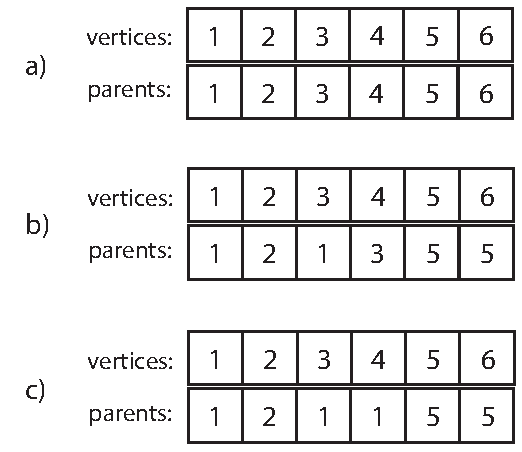
\includegraphics[width=0.7\textwidth]{Bilder/cc_steps.pdf}
	\caption{Steps of connected components with initial setup (a), first step (b) and second step (c)}
	\label{cc_steps_figure}
\end{figure}

\autoref{cc_steps_figure} a) shows the initial setup for the connected components algorithm according to the example graph of \autoref{cc_figure}: Each vertex has a parent component attribute assigned to it that is initially set to the vertex itself. For each edge in the graph, the component of the target vertex component is set to the component of the source vertex if the target component is greater than the source component in \autoref{cc_steps_figure} b). Pointer-jumping (\texttt{parent[vertex]} $\gets$ \texttt{parent[parent[vertex]]}) is then performed in \autoref{cc_steps_figure} c) so that each vertex either points to itself or to another vertex that points to itself. It is worth to note that, because edge-lists can be traversed in arbitrary order, the component of \textit{vertex 4} in the first algorithm step can also be \textit{2}. In this case, the pointer-jumping step will not perform any changes. After a second iteration, the component of \textit{vertex 2} will be set to \textit{1} resulting in termination of the algorithm.\\

The described algorithm is optimized using communication coalescing explained in \autoref{comm_coal_section}. The resulting algorithm can be seen in \autoref{cc_algorithm}. The components of the target vertices of all edges local to each processor are gathered in a bulk communication step. This data is used to set the parent component of each target's parent to the source's parent component in another bulk communication step. Pointer jumping is then performed in a synchronized way in order to allow for communication coalescing: The component of each vertex is updated and the pointers are not immediately followed but rather updated in the next iteration. The algorithm stops if there are no changes in the parent components of all vertices in an iteration. 

\begin{center}
\begin{algorithm}[h]
 \KwData{reference \textit{G} to the graph}
 \While{1}{
   \textit{gr} $\gets$ $0$\;
   \textit{i} $\gets$ $0$\;
   \For{all local out-edges $e$ in $G$} {
     \textit{indices}[i] $\gets$ global iterator position of $e.target()$\;
     ++\textit{i}\;
   }
   $data \gets $ parent components of $indices$ (communication coalescing step)\;
   \textit{i} $\gets$ $0$\;
   \For{all local out-edges $e$ in $G$} {
     $source\_parent \gets$ parent component of $e.source()$\;
     $target\_parent \gets$ parent component of $e.target()$\;
     \If{$source\_parent$ \textless{} $target\_parent$} {
       \textit{set\_data}[i] $\gets$ (global iterator position of $target\_parent$, $source\_parent$)\;
       \textit{gr} $\gets$ $1$\;
     }
     ++\textit{i}\;
   }
   update components with $set\_data$ (communication coalescing step)\;
   allreduce($gr$, ADD)\;
   \textbf{if} $gr = 0$ \textbf{then} break\;
   \While{1}{
     \textit{pj} $\gets$ $0$\;
     \textit{i} $\gets$ $0$\;
     \For{all local vertices $v$ in $G$} {
       $vertex\_parent \gets$ parent component of $v$\;
       \textit{indices}[i] $\gets$ global iterator position of $vertex\_parent$\;
       ++\textit{i}\;
     }
     $data \gets $ parent components of $indices$ (communication coalescing step)\;
     \textit{i} $\gets$ $0$\;
     \For{all local vertices $v$ in $G$} {
       \If{component of $v \neq$ $data$[i]} {
         set parent component of $v$ to $data$[i]\;
         \textit{pj} $\gets$ $1$\;
         ++\textit{i}\;
       }
     }
     allreduce($pj$, ADD)\;
     \textbf{if} $pj = 0$ \textbf{then} break\;
   }
 }
 \caption{Connected components with communication coalescing}
 \label{cc_algorithm}
\end{algorithm}
\end{center}

\subsection{Minimum Spanning Tree}
A \textit{minimum spanning tree (MST)} is a tree structure spanning a connected component along paths of minimum edge weight \cite{ita}. The tree spans all vertices in the component and the sum of edge weights of each path is guaranteed to be minimal. The MST therefore is a subset of the graph. \autoref{mst_figure} shows a graph and its corresponding minimum spanning tree.

\begin{figure}[ht]
	\centering
  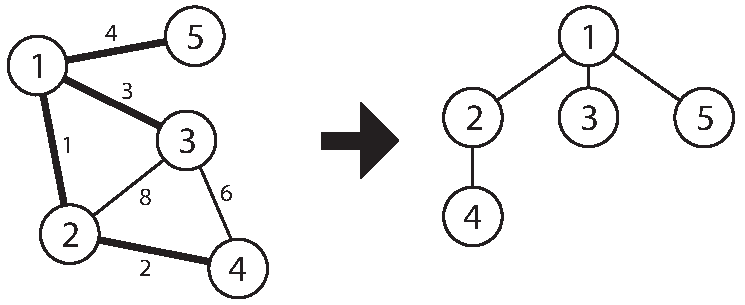
\includegraphics[width=0.8\textwidth]{Bilder/mst.pdf}
	\caption{Minimum spanning tree}
	\label{mst_figure}
\end{figure}

A graph consisting of multiple connected components contains a \textit{minimum spanning forest} of trees for each component. The algorithm presented in this section computes minimum spanning trees for all components of a graph and therefore results in a minimum spanning forest without the need of classifying the connected components beforehand.

Classical implementations of the algorithm are \textit{Kruskal's algorithm} and \textit{Prim's algorithm} \cite{prim_kruskal}. Both algorithms are greedy but have been proven to create trees with minimum edge weight.

This case study however is based on a shared-memory version of \textit{Boruvka's algorithm} \cite{boruvka} due to its increased performance in parallel environments \cite{pgas_algorithms}. It comprises iteration of three steps:

\begin{enumerate}
\item For each vertex, find the outgoing edge with the minimum weight.
\item Find connected components for the induced graph of the found edges.
\item Compact each connected component into a supervertex.
\end{enumerate}

\begin{figure}[ht]
	\centering
  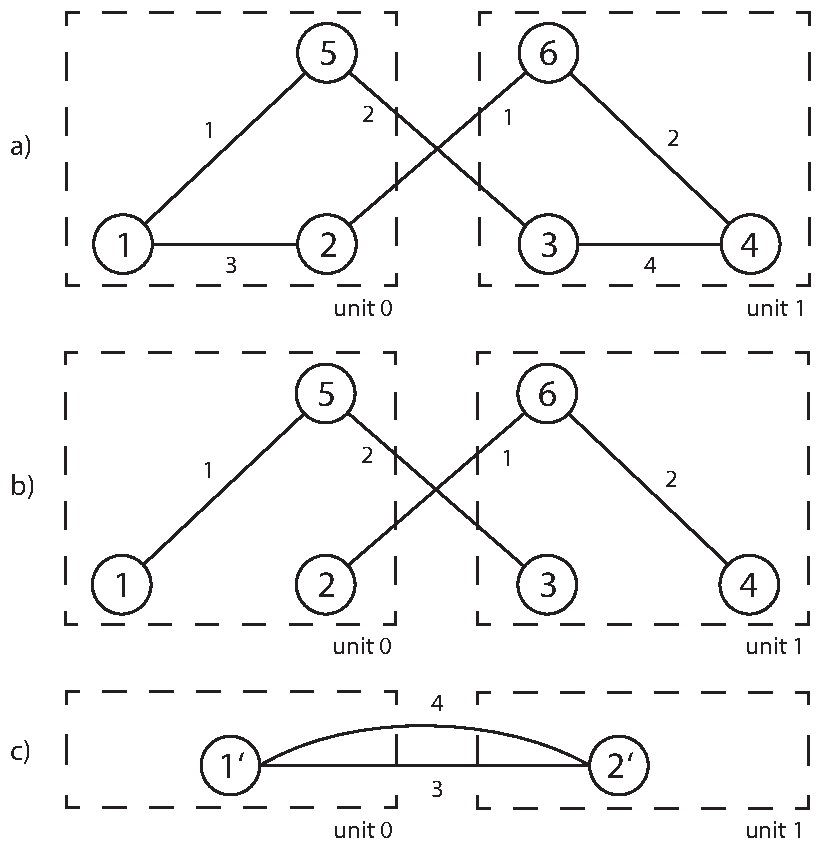
\includegraphics[width=0.8\textwidth]{Bilder/mst_boruvka.pdf}
	\caption{Distributed minimum spanning tree example showing the graph (a), the first iteration (b) and the second iteration (c) \cite{boruvka}}
	\label{mst_boruvka_figure}
\end{figure}

Each new iteration is computed on a graph composed of \textit{supervertices} which contain all edges of their respective vertices. Because compacting vertices is costly, vertices are simply labeled with their supervertex index. To find the outgoing minimum weight edge of a supervertex, multiple vertices have to be iterated over. 

Since these vertices can reside on different processors, there has to be consensus between multiple processors about the minimum weight edge. This is achieved by computing the minimum weight edge on each processor individually and then exchanging the computed edges along with their weight between all participating processors. Each processor can then determine the edge with the minimum weight and the processor it belongs to updates the edge accordingly.\\

\autoref{mst_boruvka_figure} a) depicts an exemplary graph that is distributed among two processors. \autoref{mst_boruvka_figure} b) shows the first iteration of the algorithm: For each vertex, the edges with minimum weight are chosen. The resulting connected components (1, 3, 5) and (2, 6, 4) are then compacted to the new supervertices 1' and 2' which are shown in \autoref{mst_boruvka_figure} c). Because processor 1 and processor 2 see different edges between these supervertices, both processors choose a different edge as a candidate for the minimum weight edge between the them. To reach consensus, both processors exchange these edges along with their weight and the processor owning the edge with minimum weight updates the minimum spanning tree.\\

The MST algorithm of this case study can be seen in \autoref{mst_algorithm}. It is similar to \autoref{cc_algorithm} but uses adjacency iteration to determine the minimum weight edge for each (super)vertex.

\begin{center}
\begin{algorithm}[h]
 \KwData{reference \textit{G} to the graph}
 \While{1}{
   \textit{gr} $\gets$ $0$\;
   \textit{i} $\gets$ $0$\;
   \For{all local vertices $v$ in $G$} {
     \For{all local out-edges $e$ of $v$} {
       \textit{indices}[i] $\gets$ global iterator position of $e.target()$\;
       ++\textit{i}\;
     }
   }
   $data \gets $ parent components of $indices$ (communication coalescing step)\;
   \textit{i} $\gets$ $0$\;
   \For{all local vertices $v$ in $G$} {
     \For{all local out-edges $e$ of $v$} {
       $source\_parent \gets$ parent component of $e.source()$\;
       $target\_parent \gets$ parent component of $e.target()$\;
       \If{$source\_parent \neq target\_parent \land e$ = edge with minimum weight} {
         \textit{set\_data}[global iterator position of $source\_parent]$ $\gets$ ($target\_parent$, $e$)\;
         \textit{set\_data}[global iterator position of $target\_parent]$ $\gets$ ($source\_parent$, $e$)\;
         \textit{gr} $\gets$ $1$\;
       }
       ++\textit{i}\;
     }
   }
   update components with $set\_data$ (communication coalescing step):
     if multiple edges for the same (supervertex, supervertex) pair exist, update the edge with the minimum weight\;
   allreduce($gr$, ADD)\;
   \textbf{if} $gr = 0$ \textbf{then} break\;
   \While{1}{
     \textit{pj} $\gets$ $0$\;
     \textit{i} $\gets$ $0$\;
     \For{all local vertices $v$ in $G$} {
       $vertex\_parent \gets$ parent component of $v$\;
       \textit{indices}[i] $\gets$ global iterator position of $vertex\_parent$\;
       ++\textit{i}\;
     }
     $data \gets $ parent components of $indices$ (communication coalescing step)\;
     \textit{i} $\gets$ $0$\;
     \For{all local vertices $v$ in $G$} {
       \If{component of $v \neq$ $data$[i]} {
         set parent component of $v$ to $data$[i]\;
         \textit{pj} $\gets$ $1$\;
         ++\textit{i}\;
       }
     }
     allreduce($pj$, ADD)\;
     \textbf{if} $pj = 0$ \textbf{then} break\;
   }
 }
 \caption{Minimum spanning tree with communication coalescing}
 \label{mst_algorithm}
\end{algorithm}
\end{center}

\chapter{Evaluation}
\label{eval_section}
To examine the performance and functionality of the graph concepts, the reference implementation is evaluated on a live HPC system with various kernels as described in detail in this chapter.\\

The testing environment consists of the \textit{SuperMUC Phase 2}\footnote[2]{\url{https://www.lrz.de/services/compute/supermuc/systemdescription/}} system at the \textit{Leibniz Supercomputing Centre} in Munich. It comprises \textit{six islands} composed of \textit{512 nodes} each. The nodes are interconnected with an \textit{Infiniband FDR14} network and contain two \textit{Intel Xeon E5-2697 v3} processors and 64GB of RAM.

All tests are performed on a single island with a varying amount of nodes. Because the load on the network inside the islands might vary depending on other jobs currently running on the system, each test is performed 10 times and a mean is calculated from the results.

\section{Micro-benchmarks}
This section presents a performance analysis of specific parts of the graph concepts. Because the concepts do not require inbound edge-lists in implementations of \textit{directed graph containers}, the micro-benchmarks in this section are performed on two different graph implementations to examine the difference an additional inbound edge-list imposes on performance. 

Since element deletion is currently not implemented in the reference implementation, no micro-benchmarking could be performed in this regard.

\subsection{Element creation}
Elements are strictly created on local machines. As no communication is performed during this micro-benchmark, the tests are performed on a single node with a varying amount of elements.

\subsection{Attribute access}
Attribute values of elements can be accessed on local as well as remote nodes. This test aims to highlight the differences in access times for read operations with a varying amount of elements and nodes. 

\subsection{Attribute mutation}
Attribute values of elements can be changed on local as well as remote nodes. This test aims to highlight the differences in access times for write operations with a varying amount of elements and nodes.

\subsection{Local iteration}
Iteration over local elements does not have any dependencies with remote nodes. This test is therefore performed on a single node with a varying amount of elements.

\subsection{Global iteration}
Iteration over elements stored on multiple nodes requires additional information that can degrade performance in comparison to local iteration. This test aims to highlight the differences between global and local iteration in terms of runtime. It is performed with a varying amount of nodes and a varying amount of elements.

\subsection{Memory space synchronization}
The memory space synchronization is performed between all participating nodes and requires additional communication for edges if inbound edge-lists are implemented: The edges have to be replicated to the node owning the target vertex. This test examines the runtime of the synchronization process with a varying amount of elements and nodes.

\section{Case studies}
The case studies presented in \autoref{case_studies_section} are evaluated against their UPC counterparts \cite{pgas_algorithms} in this section. Because Cong et al. used a different HPC setup for their evaluation, the resulting numbers can not be considered as directly comparable.

\subsection{Graph setup}
This section describes the properties of \texttt{dash::Graph} used for the examined case studies.

\begin{tabularx}{1\textwidth}{| l | l | X |}
  \hline
  \textbf{Property} & \textbf{Value} \\
  \endhead
  \hline
  Graph type & Directed graph\\ \hline
  Vertex attributes & - Parent component \\ \hline
  Edge attributes &  \\ \hline
  \caption{Graph setup for connected components}
\end{tabularx}

\begin{tabularx}{1\textwidth}{| l | l | X |}
  \hline
  \textbf{Property} & \textbf{Value} \\
  \endhead
  \hline
  Graph type & Undirected graph\\ \hline
  Vertex attributes & - Parent component \\ \hline
  Edge attributes & - Weight \\ \hline
  \caption{Graph setup for minimum spanning tree}
\end{tabularx}

\subsection{Input data}
To maintain comparability, the input graphs of the case studies discussed in this chapter are generated in roughly the same way as described in \cite{pgas_algorithms}. The graphs are generated using a hybrid generation scheme: 50\% of the edges are generated randomly, the rest of the edges is generated using an RMAT graph generator \cite{rmat}.

Because Cong et al. do not specify the exact input variables for the RMAT generator in their paper, default values are chosen: 

\begin{tabularx}{1\textwidth}{| l | l | X |}
  \hline
  \textbf{Variable} & \textbf{Value} \\
  \endhead
  \hline
  a & 0.57 \\ \hline
  b & 0.19 \\ \hline
  c & 0.19 \\ \hline
  d & 0.05 \\ \hline
  \caption{Input variables for RMAT graph generator}
\end{tabularx}

The generated graphs have a total of approximately \textit{100 million vertices} and \textit{400 million edges}.

\subsection{Experimental results (connected components)}

\subsection{Experimental results (minimum spanning tree)}

\chapter{Conclusion}
\section{Summary}
\section{Assessment}
\section{Outlook}


\begin{appendices}
\chapter{Graph container concepts}
\label{concept_appendix}

\section{Graph}
A \texttt{Graph} is a container providing minimal functionality for the creation and adjacency iteration of a graph data structure.

\subsection{Requirements}
\begin{itemize}
\item $X$, the graph type
\item $P$, a pair type satisfying the STL \texttt{pair} concept
\item $C$, a container type satisfying the STL \texttt{SequenceContainer} concept
\item $x$, a value of type X
\item $it_1$ and $it_2$, \texttt{InputIterators}\footnote[2]{see \autoref{stl_iterator_section}} with a valid range $[it_1, it_2]$ referring to elements of type \texttt{P<int, int>}
\item $it_v$, a value of type \texttt{X::global\_vertex\_iterator}
\item $lit_v$, a value of type \texttt{X::local\_vertex\_iterator}
\item $it_e$, a value of type \texttt{X::global\_edge\_iterator}
\item $lit_e$, a value of type \texttt{X::local\_edge\_iterator}
\end{itemize}

\subsection{Types}
\begin{tabularx}{1\textwidth}{| X | X | X |}
  \hline
  \textbf{Name} & \textbf{Type} & \textbf{Notes} \\ 
  \endhead  
  \hline
  $vertex\_type$ & a model describing vertex information &  \\ \hline
  $edge\_type$ & a model describing edge information &  \\ \hline
  $vertex\_proxy\_type$ & a proxy type encapsulating methods for the retrieval and modification of vertex data &  \\ \hline
  $edge\_proxy\_type$ & a proxy type encapsulating methods for the retrieval and modification of edge data &  \\ \hline
  $vertex\_size\_type$ & unsigned integer &  \\ \hline
  $edge\_size\_type$ & unsigned integer &  \\ \hline
  $vertex\_container\_type$ & C & user-specified STL-compatible container with contiguous range \\ \hline
  $edge\_container\_type$ & C & user-specified STL-compatible container with contiguous range \\ \hline
  $global\_vertex\_iterator$ & iterator pointing to elements of type \texttt{vertex\_type} & global iterator type satisfying \texttt{InputIterator} \\ \hline
  $local\_vertex\_iterator$ & iterator pointing to elements of type \texttt{vertex\_type} & local iterator type satisfying \texttt{InputIterator} \\ \hline
  $global\_out\_edge\_iterator$ & iterator pointing to elements of type \texttt{edge\_type} & global iterator satisfying \texttt{InputIterator} \\ \hline
  $local\_out\_edge\_iterator$ & iterator pointing to elements of type \texttt{edge\_type} & local iterator satisfying \texttt{InputIterator} \\ \hline
\end{tabularx}

\subsection{Methods and operators}
\begin{tabularx}{1\textwidth}{| l | l | X |}
  \hline
  \textbf{Expression} & \textbf{Return} & \textbf{Semantics} \\
  \endhead
  \hline
  $X(n_v, it_1, it_2)$ &  & constructs the graph holding $n_v$ vertices and std::distance($it_1$, $it_2$) edges given by the iterators $it_1$ and $it_2$ of an edge list container\\ \hline
  $x.operator[](it_v)$ & vertex\_proxy\_type & vertex identified by $it_v$ \\ \hline
  $x.operator[](lit_v)$ & vertex\_proxy\_type & vertex identified by $lit_v$ \\ \hline
  $x.operator[](it_e)$ & edge\_proxy\_type & edge identified by $it_e$ \\ \hline
  $x.operator[](lit_e)$ & edge\_proxy\_type & edge identified by $lit_e$ \\ \hline
  $x.vertices().begin()$ & global\_vertex\_iterator & iterator to the first vertex in global iteration space \\ \hline
  $x.vertices().end()$ & global\_vertex\_iterator & iterator past the last vertex in global iteration space \\ \hline
  $x.vertices().lbegin()$ & local\_vertex\_iterator & iterator to the first vertex in local iteration space \\ \hline
  $x.vertices().lend()$ & local\_vertex\_iterator & iterator past the last vertex in local iteration space \\ \hline
  $x.out\_edges().begin()$ & global\_out\_edge\_iterator & iterator to the first outbound edge in global iteration space \\ \hline
  $x.out\_edges().end()$ & global\_out\_edge\_iterator & iterator past the last outbound edge in global iteration space \\ \hline
  $x.out\_edges().lbegin()$ & local\_out\_edge\_iterator & iterator to the first outbound edge in local iteration space \\ \hline
  $x.out\_edges().lend()$ & local\_out\_edge\_iterator & iterator past the last outbound edge in local iteration space \\ \hline
  $x[it_v].out\_edges().begin()$ & global\_out\_edge\_iterator & iterator pointing to the first element in the edge-list of the vertex pointed to by $it_v$ \\ \hline
  $x[it_v].out\_edges().end()$ & global\_out\_edge\_iterator & iterator pointing past the last element in the edge-list of the vertex pointed to by $it_v$ \\ \hline
  $x[lit_v].out\_edges().lbegin()$ & local\_out\_edge\_iterator & iterator pointing to the first element in the edge-list of the vertex pointed to by $lit_v$ \\ \hline
  $x[lit_v].out\_edges().lend()$ & local\_out\_edge\_iterator & iterator pointing past the last element in the edge-list of the vertex pointed to by $lit_v$ \textcolor{red}{ONLY FOR LOCAL ITERATORS?} \\ \hline
\end{tabularx}

\subsubsection{Conditions}
\begin{tabularx}{1\textwidth}{| l | X | X |}
  \hline
  \textbf{Expression} & \textbf{Precondition} & \textbf{Postcondition} \\
  \endhead
  \hline
  $X(n_v, it_1, it_2)$ & $n_v$ = the amount of different integer values in elements of $[it_1, it_2]$ & std::distance(x.vertices().\newline begin(), x.vertices().end()) == $n_v$\newline std::distance(x.out\_edges().\newline  begin(), x.out\_edges().end()) == $n_e$\\ \hline
  $x.operator[](it_v)$ &  & vertex identified by $it_v$ \\ \hline
  $x.operator[](lit_v)$ &  & vertex identified by $lit_v$ \\ \hline
  $x.operator[](it_e)$ &  & edge identified by $it_e$ \\ \hline
  $x.operator[](lit_e)$ &  & edge identified by $lit_e$ \\ \hline
  $x.vertices().begin()$ & & \\ \hline
  $x.vertices().end()$ & & \\ \hline
  $x.vertices().lbegin()$ & & \\ \hline
  $x.vertices().lend()$ & & \\ \hline
  $x.out\_edges().begin()$ & & \\ \hline
  $x.out\_edges().end()$ & & \\ \hline
  $x.out\_edges().lbegin()$ & & \\ \hline
  $x.out\_edges().lend()$ & & \\ \hline
  $x[it_v].out\_edges().begin()$ & & \\ \hline
  $x[it_v].out\_edges().end()$ & & \\ \hline
  $x[lit_v].out\_edges().lbegin()$ & & \\ \hline
  $x[lit_v].out\_edges().lend()$ & & \\ \hline
\end{tabularx}

\section{DynamicGraph}
A \texttt{DynamicGraph} is a \texttt{Graph} that enables dynamic addition and removal of vertices and edges.

\subsection{Requirements}
\begin{itemize}
\item $X$, the graph type
\item $P$, a pair type satisfying the STL \texttt{pair} concept
\item $x$, a value of type X
\item $n_v$, a value of type \texttt{X::vertex\_size\_type}
\item $n_e$, a value of type \texttt{X::edge\_size\_type}
\item $it_v$, a value of type \texttt{X::global\_vertex\_iterator}
\item $lit_v$, $lit_{v1}$ and $lit_{v2}$, values of type \texttt{X::local\_vertex\_iterator}
\item $it_e$, a value of type \texttt{X::global\_out\_edge\_iterator}
\item $lit_e$, a value of type \texttt{X::local\_out\_edge\_iterator}
\end{itemize}

\subsection{Methods and operators}
\begin{tabularx}{1\textwidth}{| l | l | X |}
  \hline
  \textbf{Expression} & \textbf{Return} & \textbf{Semantics} \\
  \endhead  
  \hline
  $X(n_v, n_e)$ &  & constructs the graph with reserved memory for $n_v$ vertices and $n_v * n_e$ edges \\ \hline
  $x.add\_vertex()$ & local\_vertex\_iterator & adds a vertex \\ \hline
  $x.remove\_vertex(it_v)$ &  & removes a vertex pointed to by $it_v$ \\ \hline
  $x.remove\_vertex(lit_v)$ &  & removes a vertex pointed to by $lit_v$ \\ \hline
  $x.add\_edge(lit_{v1}, lit_{v2})$ & P\textless local\_out\_edge\_iterator, bool\textgreater & adds an edge between vertices pointed to by $lit_{v1}$ and $lit_{v2}$ and returns whether the edge has been added \\ \hline
  $x.add\_edge(lit_v, it_{v})$ & P\textless local\_out\_edge\_iterator, bool\textgreater & adds an edge between vertices pointed to by $lit_v$ and $it_{v}$ and returns whether the edge has been added \\ \hline
  $x.remove\_edge(it_e)$ &  & removes an edge identified by $it_e$ \\ \hline
  $x.remove\_edge(lit_e)$ &  & removes an edge identified by $lit_e$ \\ \hline
  $x.commit()$ &  & synchronizes memory space across all processors \\ \hline
\end{tabularx}

\subsubsection{Conditions}
\begin{tabularx}{1\textwidth}{| l | X | X |}
  \hline
  \textbf{Expression} & \textbf{Precondition} & \textbf{Postcondition} \\
  \endhead  
  \hline
  $X(n_v, n_e)$ & & memory allocated for $n_v$ vertices and $n_v * n_e$ edges \\ \hline
  $x.add\_vertex()$ &  & returned iterator points to constructed vertex in global iteration space \\ \hline
  $x.remove\_vertex(it_v)$ & $it_v$ points to a valid vertex in X & \\ \hline
  $x.remove\_vertex(lit_v)$ & $lit_v$ points to a valid vertex in X & \\ \hline
  $x.add\_edge(lit_{v1}, lit_{v2})$ & $lit_{v1}$ and $lit_{v2}$ point to valid vertices in X & returned index identifies constructed edge in global index space \\ \hline
  $x.add\_edge(lit_v, it_{v}$) & $it_{v}$ and $lit_v$ point to valid vertices in X & returned index identifies constructed edge in global index space \\ \hline
  $x.remove\_edge(it_e)$ & $it_e$ points to a valid edge in X & \\ \hline
  $x.remove\_edge(lit_e)$ & $lit_e$ points to a valid edge in X & \\ \hline
  $x.commit()$ & & locally added elements published in global address space,\newline global iteratos are invalidated \\ \hline
\end{tabularx}

\section{AttributedGraph}
An \texttt{AttributedGraph} is a \texttt{Graph} containing arbitrary attributes for vertices and edges.

\subsection{Requirements}
\begin{itemize}
\item $X$, the graph type
\item $VT$, a vertex attribute type
\item $ET$, an edge attribute type
\item $TP$, a tuple type satisfying the STL \texttt{tuple} concept
\item $P$, a pair type satisfying the STL \texttt{pair} concept
\item $x$, a value of type X
\item $n_v$, a value of type \texttt{X::vertex\_size\_type}
\item $it_1$ and $it_2$, \texttt{InputIterators} with a valid range $[it_1, it_2]$ referring to elements of type \texttt{TP<P<int, VT>, P<int, VT>, ET>}
\item $it_v$, a value of type \texttt{X::global\_vertex\_iterator}
\item $lit_v$, a value of type \texttt{X::local\_vertex\_iterator}
\item $it_e$, a value of type \texttt{X::global\_out\_edge\_iterator}
\item $lit_e$, a value of type \texttt{X::local\_out\_edge\_iterator}
\item $a_v$, a value of type \texttt{X::vertex\_attributes\_type}
\item $a_e$, a value of type \texttt{X::edge\_attributes\_type}
\end{itemize}

\subsection{Types}
\begin{tabularx}{\textwidth}{| X | X | X |}
  \hline
  \textbf{Name} & \textbf{Type} & \textbf{Notes} \\ 
  \endhead  
  \hline
  $vertex\_attributes\_type$ & VT & user-specified static struct \\ \hline
  $edge\_attributes\_type$ & ET & user-specified static struct \\ \hline
\end{tabularx}

\subsection{Methods and operators}
\begin{tabularx}{1\textwidth}{| l | l | X |}
  \hline
  \textbf{Expression} & \textbf{Return} & \textbf{Semantics} \\
  \endhead  
  \hline
  $X(n_v, it_1, it_2)$ &  & constructs the graph holding $n_v$ vertices and std::distance($it_1$, $it_2$) edges given by the iterators $it_1$ and $it_2$ of an edge list container\\ \hline
  $x[it_v].attributes()$ & $vertex\_attributes\_type$ & returns the attributes of the vertex pointed to by $it_v$\\ \hline
  $x[lit_v].attributes()$ & $vertex\_attributes\_type$ & returns the attributes of the vertex pointed to by $lit_v$\\ \hline
  $x[it_e].attributes()$ & $edge\_attributes\_type$ & returns the attributes of the edge pointed to by $it_e$\\ \hline
  $x[lit_e].attributes()$ & $edge\_attributes\_type$ & returns the attributes of the edge pointed to by $lit_e$\\ \hline
  $x[it_v].set\_attributes(a_v)$ &  & replaces the attributes of the vertex pointed to by $it_v$ with a copy of $a_v$\\ \hline
  $x[lit_v].set\_attributes(a_v)$ &  & replaces the attributes of the vertex pointed to by $lit_v$ with a copy of $a_v$\\ \hline
  $x[it_e].set\_attributes(a_e)$ &  & replaces the attributes of the edge pointed to by $it_e$ with a copy of $a_e$\\ \hline
  $x[lit_e].set\_attributes(a_e)$ &  & replaces the attributes of the edge pointed to by $lit_e$ with a copy of $a_e$\\ \hline
\end{tabularx}

\subsubsection{Conditions}
\begin{tabularx}{1\textwidth}{| l | X | X |}
  \hline
  \textbf{Expression} & \textbf{Precondition} & \textbf{Postcondition} \\
  \endhead  
  \hline
  $X(n_v, it_1, it_2)$ &  & memory allocated for $n_v$ vertices and std::distance($it_1$, $it_2$) edges\\ \hline
  $x[it_v].attributes()$ & $it_v$ points to a valid vertex in X & \\ \hline
  $x[lit_v].attributes()$ & $lit_v$ points to a valid vertex in X & \\ \hline
  $x[it_e].attributes()$ & $it_e$ points to a valid edge in X & \\ \hline
  $x[lit_e].attributes()$ & $lit_e$ points to a valid edge in X & \\ \hline
  $x[it_v].set\_attributes(a_v)$ & $it_v$ points to a valid vertex in X & \\ \hline
  $x[lit_v].set\_attributes(a_v)$ & $lit_v$ points to a valid vertex in X & \\ \hline
  $x[it_e].set\_attributes(a_e)$ & $it_e$ points to a valid edge in X & \\ \hline
  $x[lit_e].set\_attributes(a_e)$ & $lit_e$ points to a valid edge in X & \\ \hline
\end{tabularx}

\section{DuplexGraph}
A \texttt{DuplexGraph} is a \texttt{Graph} with iterators for inbound edges for each vertex. A container supporting undirected graphs is necessarily a \texttt{DuplexGraph}. For directed graphs, inbound edge iterators are optional.

\subsection{Requirements}
\begin{itemize}
\item $X$, the graph type
\item $x$, a value of type X
\item $it_v$, a value of type \texttt{X::global\_vertex\_iterator}
\item $lit_v$, a value of type \texttt{X::local\_vertex\_iterator}
\end{itemize}

\subsection{Types}
\begin{tabularx}{1\textwidth}{| X | X | X |}
  \hline
  \textbf{Name} & \textbf{Type} & \textbf{Notes} \\ 
  \endhead  
  \hline
  $global\_in\_edge\_iterator$ & iterator pointing to elements of type \texttt{edge\_type} & global iterator satisfying \texttt{InputIterator} \\ \hline
  $local\_in\_edge\_iterator$ & iterator pointing to elements of type \texttt{edge\_type} & local iterator satisfying \texttt{InputIterator} \\ \hline
\end{tabularx}

\subsection{Methods and operators}
\begin{tabularx}{1\textwidth}{| l | l | X |}
  \hline
  \textbf{Expression} & \textbf{Return} & \textbf{Semantics} \\
  \endhead
  \hline
  $x.in\_edges().begin()$ & global\_in\_edge\_iterator & iterator to the first inbound edge in global iteration space \\ \hline
  $x.in\_edges().end()$ & global\_in\_edge\_iterator & iterator past the last inbound edge in global iteration space \\ \hline
  $x.in\_edges().lbegin()$ & local\_in\_edge\_iterator & iterator to the first inbound edge in local iteration space \\ \hline
  $x.in\_edges().lend()$ & local\_in\_edge\_iterator & iterator past the last inbound edge in local iteration space \\ \hline
  $x[it_v].in\_edges().begin()$ & global\_in\_edge\_iterator & iterator to the first inbound edge connected to the vertex pointed to by $it_v$ \\ \hline
  $x[it_v].in\_edges().end()$ & global\_in\_edge\_iterator & iterator past the last inbound edge connected to to the vertex pointed to by $it_v$ \\ \hline
  $x[lit_v].in\_edges().lbegin()$ & local\_in\_edge\_iterator & iterator to the first inbound edge connected to the vertex pointed to by $lit_v$ \\ \hline
  $x[lit_v].in\_edges().lend()$ & local\_in\_edge\_iterator & iterator past the last inbound edge connected to to the vertex pointed to by $lit_v$ \\ \hline
\end{tabularx}

\subsection{Conditions}
\begin{tabularx}{1\textwidth}{| l | X | X |}
  \hline
  \textbf{Expression} & \textbf{Precondition} & \textbf{Postcondition} \\
  \endhead
  \hline
  $x.in\_edges().begin()$ & & \\ \hline
  $x.in\_edges().end()$ & & \\ \hline
  $x.in\_edges().lbegin()$ & & \\ \hline
  $x.in\_edges().lend()$ & & \\ \hline
  $x[it_v].in\_edges().begin()$ & $it_v$ points to a valid vertex in X & \\ \hline
  $x[it_v].in\_edges().end()$ & $it_v$ points to a valid vertex in X & \\ \hline
  $x[lit_v].in\_edges().lbegin()$ & $lit_v$ points to a valid vertex in X & \\ \hline
  $x[lit_v].in\_edges().lend()$ & $lit_v$ points to a valid vertex in X & \\ \hline
\end{tabularx}

\section{CombinedEdgeGraph}
A \texttt{CombinedEdgeGraph} is a \texttt{Graph} with additional iterators for a combination of inbound and outbound edges.

\subsection{Requirements}
\begin{itemize}
\item $X$, the graph type
\item $x$, a value of type X
\item $it_v$, a value of type \texttt{X::global\_vertex\_iterator}
\item $lit_v$, a value of type \texttt{X::local\_vertex\_iterator}
\end{itemize}

\subsection{Types}
\begin{tabularx}{1\textwidth}{| l | X | X |}
  \hline
  \textbf{Name} & \textbf{Type} & \textbf{Notes} \\ 
  \endhead  
  \hline
  $global\_edge\_iterator$ & iterator pointing to elements of type \texttt{edge\_type} & global iterator satisfying \texttt{InputIterator} \\ \hline
  $local\_edge\_iterator$ & iterator pointing to elements of type \texttt{edge\_type} & local iterator satisfying \texttt{InputIterator} \\ \hline
\end{tabularx}

\subsection{Methods and operators}
\begin{tabularx}{1\textwidth}{| l | l | X |}
  \hline
  \textbf{Expression} & \textbf{Return} & \textbf{Semantics} \\
  \endhead
  \hline
  $x.edges().begin()$ & global\_edge\_iterator & iterator to the first edge (inbound and outbound) in global iteration space \\ \hline
  $x.edges().end()$ & global\_edge\_iterator & iterator past the last edge (inbound and outbound) in global iteration space \\ \hline
  $x.edges().lbegin()$ & local\_edge\_iterator & iterator to the first edge (inbound and outbound) in local iteration space \\ \hline
  $x.edges().lend()$ & local\_edge\_iterator & iterator past the last edge (inbound and outbound) in local iteration space \\ \hline
  $x[it_v].edges().begin()$ & global\_edge\_iterator & iterator to the first edge (inbound and outbound) connected to the vertex pointed to by $it_v$ \\ \hline
  $x[it_v].edges().end()$ & global\_edge\_iterator & iterator past the last edge (inbound and outbound) connected to to the vertex pointed to by $it_v$ \\ \hline
  $x[lit_v].edges().lbegin()$ & local\_edge\_iterator & iterator to the first edge (inbound and outbound) connected to the vertex pointed to by $lit_v$ \\ \hline
  $x[lit_v].edges().lend()$ & local\_edge\_iterator & iterator past the last edge (inbound and outbound) connected to to the vertex pointed to by $lit_v$ \\ \hline
\end{tabularx}

\subsection{conditions}
\begin{tabularx}{1\textwidth}{| l | X | X |}
  \hline
  \textbf{Expression} & \textbf{Precondition} & \textbf{Postcondition} \\
  \endhead
  \hline
  $x.edges().begin()$ & & \\ \hline
  $x.edges().end()$ & & \\ \hline
  $x.edges().lbegin()$ & & \\ \hline
  $x.edges().lend()$ & & \\ \hline
  $x[it_v].edges().begin()$ & $it_v$ points to a valid vertex in X & \\ \hline
  $x[it_v].edges().end()$ & $it_v$ points to a valid vertex in X & \\ \hline
  $x[lit_v].edges().lbegin()$ & $lit_v$ points to a valid vertex in X & \\ \hline
  $x[lit_v].edges().lend()$ & $lit_v$ points to a valid vertex in X & \\ \hline
\end{tabularx}

\end{appendices}

% ---------------------------------------------------------------
\backmatter % ab hier keine Nummerierung mehr
    \listoffigures
    \bibliographystyle{alphadin}
    \bibliography{./Bib/effe17}

\end{document}
